\documentclass[12pt, a4paper]{book}

% !TeX program = lualatex
% !BIB program = bibtex 

\usepackage{pacchetti}
\usepackage{enumitem} % resume in enumerate environment



\definecolor{turquoise}{RGB}{0, 247, 230}
\definecolor{goldenyellow}{RGB}{255, 218, 66}
\definecolor{fuchsia}{RGB}{255, 0, 172}

%%%%%%%%%%%%%%%%%%%%%%%%%%%%%%%%%%%%%%% HEAD COMMANDS	
\newtheorem{theorem}{Theorem}[section]

\newtheorem{corollary}[theorem]{Corollary}

\newtheorem{lemma}[theorem]{Lemma}

\newtheorem{prop}[theorem]{Proposition}

\theoremstyle{definition}
\newtheorem{definition}{Definition}[section]

\theoremstyle{remark}
\newtheorem*{remark}{Remark}

\newcommand{\EAK}[1]{\textcolor{red}{EAK: #1}}
\newcommand{\VS}[1]{\textcolor{cyan}{VS: #1}}

%%%%%%%%%%%%%%%%%%%%%%%%%%%%%%%%%%%%%%% MATH SYMBOLS
\newcommand{\R}{{\mathbb{R}}}
\newcommand{\N}{{\mathbb{N}}}

 \newcommand{\pprec}{\prec\mathrel{\mkern-5mu}\prec}






\title{Master Thesis}

\author{Veronica Sacchi\thanks{veronica.sacchi@sns.it}\\
Supervisor: Eleni A. Kontou\thanks{e.a.kontou@uva.nl}}

% Bibliografia
\usepackage[backend=bibtex,doi=false,isbn=false,url=false]{biblatex}
\addbibresource{bibliografia.bib}

\begin{document}

\maketitle

\tableofcontents
\clearpage

\chapter*{Notation and Conventions}
\thispagestyle{empty}
%nice frame
\usetikzlibrary{math,calc,decorations.pathmorphing}
\tikzset{
	fancy corner/.pic={
\textit{}		\draw (0,4) -- (0,2.5) to[bend left] (2.5,0) -- (4,0);
		\draw (0.5,4) -- (0.5,0.5) -- (4,0.5);
		\draw (1,4) -- (1,0) -- (0,0) -- (0,1) -- (4,1);
	},
	fancy edge/.pic={
		\draw (1,0) -- (0,1) -- (-1,0) -- (0,-1) -- cycle;
		\fill[red] (1,0) circle(.5pt);
		\def\a{.7}
		\foreach \xs in {1,-1} {
			\begin{scope}[xscale=\xs,shift={(.2,0)}]
				\draw (4,0) -- ({1+\a},0) -- (1,\a) -- ({1-\a},0) -- (1,{-\a}) -- ({1+\a},0);
				\foreach \ys in {1,-1} {
					\draw[yscale=\ys] (4,0.5) -- ({0.5*(3+\a)},0.5) -- +(135:0.6);
				}
			\end{scope}
		}
		\fill (0,0) circle (.2);
	},
	pics/fancy rectangle/.style n args={4}{code={
			\pic at (#1,#3) {fancy corner};
			\pic[yscale=-1] at (#1,#4) {fancy corner};
			\pic[xscale=-1] at (#2,#3) {fancy corner};
			\pic[xscale=-1,yscale=-1] at (#2,#4) {fancy corner};
			\pic at ({(#1+#2)/2},{#3+.5}) {fancy edge};
			\pic at ({(#1+#2)/2},{#4-.5}) {fancy edge};
			\foreach \i in {0,0.5,1} {
				\foreach \y in {#3,#4-1} {
					\draw ({#1+3.9},{\y+\i}) -- ({#1+#2)/2-3.9},{\y+\i});
					\draw ({#2-3.9},{\y+\i}) -- ({#1+#2)/2+3.9},{\y+\i});
				}
				\foreach \x in {#1,#2-1} {
					\draw ({\x+\i},{#3+3.9}) -- ({\x+\i},{#4-3.9});
			}}
	}},
}

\def\decorationscale{.5} % decoration scale
\colorlet{decoration color}{turquoise!70} % decoration color

	\begin{tikzpicture}[draw=decoration color,fill=decoration color,line width=2pt,remember picture,overlay,x={(\decorationscale,0)},y={(0,\decorationscale)}]
	\tikzmath{
		coordinate \ne,\sw;
		\ne=(current page.north east)+(-1cm,-1cm);
		\sw=(current page.south west)+(1cm,1cm);
		\xx=(\swx/1cm)/\decorationscale;
		\xxx=\nex/1cm/\decorationscale;
		\yy=\swy/1cm/\decorationscale;
		\yyy=\ney/1cm/\decorationscale;
	}
	\pic{fancy rectangle={\xx}{\xxx}{\yy}{\yyy}};
	\end{tikzpicture}

In this work we are going to use the \([-, + , +]\) conventions as labelled in the Misner, Thorne and Wheeler \cite{misner1973gravitation}. That means:
\begin{itemize}
	\item[\ding{99}] The metric signature is \((+, -, -, -)\).
	\item[\ding{99}]  The Riemann tensor in components is defined as:
	\[
	R\indices{^{\mu}_{\nu\alpha\beta}} = \partial_{\alpha}\Gamma^{\mu}_{\nu\beta} - \partial_{\beta}\Gamma^{\mu}_{\nu\alpha} + \Gamma^{\mu}_{\alpha\tau}\Gamma^{\tau}_{\nu\beta} - \Gamma^{\mu}_{\beta\tau}\Gamma^{\tau}_{\nu\alpha}.
	\]
	In particular, it's true that:
	\[
	[\nabla_U, \nabla_V] W^{\mu} = R\indices{^{\mu}_{\nu\alpha\beta}}W^{\nu}U^{\alpha}V^{\beta}.
	\]
	\item[\ding{99}]  Einstein equations are \(R_{\mu\nu} - \frac{1}{2}Rg_{\mu\nu} = 8\pi T_{\mu\nu}\).
\end{itemize}

\begin{tikzpicture}
	\draw [fill=turquoise,turquoise] (0,0) rectangle (1,1);
	\draw [fill=goldenyellow,goldenyellow] (1,0) rectangle (2,1);
	\draw [fill=fuchsia,fuchsia] (2,0) rectangle (3,1);
	\draw [fill=turquoise,turquoise] (3,0) rectangle (4,1);
\end{tikzpicture}

\chapter{Fundamental Concepts}
\section{Geodesics}
The main source of inspiration for this first chapter is the book by B. O'Neill \cite{o1983semi}. We shall refer mainly to chapters \(10\) and \(14\); when needed, more specific references will be made.

Let's start off with some basic concepts derived from differential geometry. We will generally address the spacetime manifold as \(M\), \(g\) its Lorentizan metric and \(\nabla\) the Levi-Civita connection.
We will generally assume that a \emph{spacetime} is a smooth, time-oriented Lorentzian manifold; we will use the terms manifold and spacetime intercheangeably, unless otherwise stated.
The first fundamental definiton we need is:
\begin{definition}
	Let \((M, g)\) be a spacetime and \(I \subseteq \R\) an interval; a smooth curve \(\gamma : I \rightarrow M\) is a \emph{geodesic} if its tangent field is parallel transported along \(\gamma\).\\
\end{definition}    

Calling \(U\indices{^{\mu}} \coloneqq \dot{\gamma}^{\mu}\) the tangent field, this definition is equivalent to the equation:
\[
\nabla_U U^{\mu} \coloneqq \frac{D\tensor{U}{^\mu} }{dt} \equiv 0.
\]


A \emph{curve} is a \(1\)-parameter map; similarly we can define a \emph{family of curves} as a \(2\)-parameter map \(\zeta: I \times J \rightarrow M\), where \(I, J \subseteq \R\) are intervals. This gives us \(2\) tangent fields, which we call respectively \emph{longitudinal} and \emph{transverse}:
\[
U^{\mu} \coloneqq \frac{\partial}{\partial t} \zeta^{\mu}(t,s); \quad \quad \quad 
V^{\mu} \coloneqq \frac{\partial}{\partial s} \zeta^{\mu}(t,s). 
\]

\begin{definition}
	Given a curve \(\gamma\), a \emph{(smooth) variation of \(\gamma\)} is any (smooth) \(2\)-parameter map \(\zeta(s,t)\) such that 
	\[
	\left. \zeta(s, t) \right\vert_{s = 0} = \gamma(t).
	\]
\end{definition}

%todo: metti un bel disegno di una famigla di curve

\begin{remark}
	Commutation of partial derivatives immediately gives 
	\[
	[U, V] = 0 \implies \nabla_U V^{\mu} = \nabla_V U^{\mu}
	\]
	and, by definition of the Riemann tensor
	\[
	[\nabla_U, \nabla_V]W^{\mu} = R\indices{^{\mu}_{\nu\alpha\beta}}W^{\nu}U^{\alpha}V^{\beta}
	\]
\end{remark}

By this remark we can compute the second derivative of the transverse field:
\[
\frac{D^2\tensor{V}{^\mu} }{dt^2} = \nabla_U\nabla_V U^{\mu} = \nabla_V\nabla_U U^{\mu} + R\indices{^{\mu}_{\nu\alpha\beta}}U^{\nu}U^{\alpha}V^{\beta}
\]

which his leads us to the second fundamental objects we need to define. 
\begin{definition}
	Given a family of \emph{geodesics} \(\gamma_s(t) \coloneqq \zeta(s,t)\), the transversal field \(V^{\mu} \coloneqq \frac{\partial}{\partial s} \zeta^{\mu}(t,s)\) is said to be a \emph{Jacobi field}.
\end{definition}

This vector field has a very important characterization, which here we'll only state:
\begin{lemma}
\(V^{\mu}\) is a \emph{Jacobi field} if and only if it satisfies the equation
	\[
	\frac{D^2\tensor{V}{^\mu} }{dt^2} = \nabla_U\nabla_V U^{\mu} =  R\indices{^{\mu}_{\nu\alpha\beta}}U^{\nu}U^{\alpha}V^{\beta}
	\].
\end{lemma}

\section{Submanifolds}
\label{sec:submanifolds}

\begin{definition}
	Let \(M\) be a submanifold of the semi-Riemannian manifold \(\bar{M}\), and \(j:M\rightarrow\bar{M}\) the inclusion map. Then \(M\) is a \emph{semi-Riemannian submanifold} if the pullback of the metric tensor \(j^*(g)\) is a metric tensor on \(M\).
\end{definition}

This definiton makes it clear that observers on the submanifold \(M\) agree on the notion of distance as if they were outside the submanifold. Nevertheless, observers within \(M\) see the world differently than observers from the outside: they in fact will inherit \(2\) different connections from their respective notion of metric. 

The comparison between these \(2\) different Levi-Civita connections gives surge to the \emph{second fundamental form}, which provides an infinitesimal description of the shape of \(M\) within \(\bar{M}\).

In order to introduce this important object notice first of all that:
\[
\forall p \in M \quad T_p\bar{M} = \underbrace{T_pM}_{\text{vectors tangent to }M}+ \underbrace{T_p(M)^{\perp}}_{\text{vectors othogonal to } M}
\]

\noindent and we will generally call \(\Pi_p^{\parallel}\coloneqq d_pj\) and \(\Pi_p^{\perp}\coloneqq \mathbb{1} - d_pj\) the projecive maps on these \(2\) subspaces.
Adopting a similar notation, we can decompose the set of all smooth fields in \(T\bar{M}\) restricted to \(M\) as:
\[
\bar{\mathfrak{X}}(M) = \mathfrak{X}(M) + \mathfrak{X}(M)^{\perp}.
\]

Now, the connection \(\bar{D}\) on \(\bar{M}\) will naturally give raise to a connection on \(M\)
\begin{align*}
\bar{D} : \mathfrak{X}(M) \times \bar{\mathfrak{X}}(M) & \rightarrow \bar{\mathfrak{X}}(M) \\
	 V \times X &\mapsto \bar{D}_V X
\end{align*}

by taking any smooth extension of the fields \(V\) and \(X\) to \(\mathfrak{X}(\bar{M})\), and then restricting again on \(M\). It can be proved that \(\bar{D}_V X\) is a well-defined smooth vector field on \(M\). In particular
\begin{lemma} 
	if \(V, W \in \mathfrak{X}(M)\) and \(D\) is the Levi-Civita connection on \(M\), it holds that
	\[
	D_V W = \Pi^{\parallel}\left(\bar{D}_V W\right).
	\]
\end{lemma}

It's evident then that the Levi-Civita connection on \(M\) is loosing something repect to the induced connection from \(\bar{M}\). This is precisely the object we have been looking for:
\begin{definition}
	given \(M \subset \bar{M}\) a semi-Riemannian submanifold, the \emph{shape tensor} (or \emph{second fundamental form}) is defined as:
	\begin{align*}
		\mathbb{I} : \mathfrak{X}(M) \times \mathfrak{X}(M) &\longrightarrow \mathfrak{X}(M)^{\perp}\\
							V \times W &\mapsto \Pi^{\perp}\left(\bar{D}_V W\right)
	\end{align*}
	\noindent and in particular is bilinear and symmetric.
\end{definition}

In order to gain a better understanding of what this object encodes, let's think for a moment about the following example. Given a field \(Y \in \mathfrak{X}(M)\) tangent to a curve \(\alpha\) of \(M\), parametrized by \(s\), we indicate:
\[
\dot{Y} \coloneqq \frac{\bar{D}Y}{ds} \quad \quad Y' \coloneqq \frac{DY}{ds}
\]
It is then easy to prove that:
\[
\ddot{\alpha} = \alpha'' + \mathbb{I}(\alpha', \alpha')
\]

and hence, we can think of \(\mathbb{I}\) as the additional external ``force'' needed to keep a point moving on \(M \subset \bar{M}\), a sort of costraining force. An equivalent interpretation is by how much a vector paralleled transported in \(M\) according to \(D\) is actually changing from the point of view of \(\bar{D}\).

%todo: inserisci disegno pag.103 O'Neill


The second fundamental form induces a vector field on \(M\) called \emph{mean curvature}.
\begin{definition}
		Let\(M \subset \bar{M}\) be an  \(n\)-semi-Riemannian submanifold, with \emph{shape tensor} \(\mathbb{I}\), and \(\{\textbf{e}_i\}_{i \in \{1, \ldots, n\}}\) any frame on \(M\) at \(p\). Then we call \emph{mean curvature vector field} the field \(\mathfrak{H} \in \mathfrak{X}(M)^{\perp} \) defined by:
		\[
		\mathfrak{H}^{\mu}(p) = \frac{1}{n} \sum_{i=1}^{n} \epsilon_i \mathbb{I}^{\mu}(\textbf{e}_i, \textbf{e}_i).
		\]
		where 
		\[
		\epsilon_i = 
		\begin{cases}
		+1 \quad \text{se } \textbf{e}_i \text{\`e di tipo \emph{tempo}} \\
		-1 \quad \text{se } \textbf{e}_i \text{\`e di tipo \emph{spazio}}
		\end{cases}
		\]
\end{definition}

This definition will be particularly important for the proof of Null Singularity Theorems, as they are instrumental to define the concept of a \emph{trapped surface}, the initial condition needed to eventually develop a singularity (in the classical limit). 

\section{Trapped surfaces}

\begin{definition}
	We say that a spacelike submanifold \(M\) is \emph{future-converging} provided its mean curvature vetor field \(\mathfrak{H}\) is past-pointing timelike.
\end{definition}



It is only a matter of simple linear algebra in each normal space \(T_p(M)^{\perp}\) to show that
\begin{lemma} \label{lemma:charact-trapped}
	assuming \(M\) is a \emph{spacelike} submanifold, the follwoing statements are equivalent:
	\begin{enumerate}
		\item  \(k(v) =g(\mathfrak{H}, v) < 0 \) for all future pointing \emph{null} vectors \(v\) normal to M.
		\item  \(k(w) =g(\mathfrak{H}, w) < 0 \) for all future pointing \emph{causal} vectors \(v\) normal to M.
		\item \(\mathfrak{H}\) is past-pointing timelike.
	\end{enumerate}
\end{lemma}

\begin{proof}
	We will prove a chain of implications to gain the equivalence.
	
	\(\mathbf{2) \implies 1)]}\) this is trivial because any null vector is a causal vector.
	
	\(\mathbf{1) \implies 3)]}\) Let's write \(\mathfrak{H}^{\mu} = (\mathfrak{H}^0, \vec{\mathfrak{H}})\). It is possible to choose a spacelike \(3-\)vector \(\vec{v}\) such that \(\vert\vec{v}\cdot\vec{\mathfrak{H}}\vert = - \vert\vec{v}\vert\cdot\vert\vec{\mathfrak{H}}\vert\) and  then complete it to the future-pointing null vector \(v^{\mu} = (v^0, \vec{v})\) (where \(v^0 = \vert \vec{v}\vert > 0\)).
	Now:
	\[
	\mathfrak{H}^{\mu}v_{\mu} = \mathfrak{H}^0v^0 - \vec{\mathfrak{H}}\cdot\vec{v} < 0 \quad \implies 
	\quad v^0 \mathfrak{H}^0 < - \vert\vec{v}\vert\cdot\vert\vec{\mathfrak{H}}\vert < 0
	\]
	which, for the positivity of \(v^0\), implies that \(H^{\mu}\) is timelike and past-pointing.
	
	\(\mathbf{3) \implies 2)]}\) first of all observe that any causal vector can be written as the sum of \(2\) future-pointing vectors such that \(w^{\mu}= v^{\mu} + t^{\mu}\) where \(v\) is null, and \(t^{\mu} = (t^0, \vec{0})\) (with \(t^0 \ge 0\)). At this point:
	\[
	w^{\mu}\mathfrak{H}^{\mu} = v^{\mu}\mathfrak{H}^{\mu} + \underbrace{t^0 \mathfrak{H}^0}_{\le0}
	\]
	Moreover, by Cauchy-Schwartz we have:
	\[
	v_{\mu}\mathfrak{H}^{\mu} = v^0 \mathfrak{H}^0 - \vec{\mathfrak{H}}\cdot\vec{v} \le v^0\mathfrak{H}^0 +\vert \vec{\mathfrak{H}}\vert\cdot\underbrace{\vert\vec{v}\vert}_{v^0} = v^0\underbrace{(\mathfrak{H}^0 + \vert \vec{\mathfrak{H}}\vert)}_{<0} < 0.
	\]
\end{proof}

\subsection{Causality conditions}

The notion of \emph{causality} has to do with the fact that in a Lorentzian manifold, starting from a  point \(p\) it is not true that an observer or a light ray can travel to any other point \(q\), as they are allowed only to move along (future pointing) causal geodesics (i.e. whose tangent field is never spacelike).

We will denote causality relations with the following notation, following \cite{o1983semi}.
\begin{enumerate}
	\item  \(p \guillemotleft q\) means there is a future-pointing \emph{timelike} curve in \(M\) connecting \(p\) to \(q\).
	\item \(p \prec q\) means there is a future-pointing \emph{causal} curve from \(p\) to \(q\).
\end{enumerate}

Evidently \(p\guillemotleft q\) implies \(p\prec q\) but not vice versa. For a subset \(A \subseteq M\) we also define:
\begin{enumerate}
	\item the \emph{chronological future} of \(A\)
	\[
	I^+(A) =\{ q\in M :\quad\exists p \in A\text{ with } p\guillemotleft q\}.
	\]
	\item the \emph{causal future} of \(A\)
	\[
	I^+(A) =\{ q\in M : \quad\exists p \in A\text{ with } p\prec q\}.
	\]
\end{enumerate}

%\clearpage

\chapter{Focal Points}
\label{ch:focal-points}

Now that we know what a submanifold is, an important question we might like to answer is \emph{given a submanifold \(P\subset M\) and a point \(q \notin P\), what is the ``best'' path from \(P\) to \(q\)?} 

Here ``best'' means a path that maximizes (or minimizes) some relevant functional of the curves joining \(P\) to \(q\). The most important functional we would like to study is the curve-lenght \(L[\gamma]\): it carries a powerful physical meaning but it turns out to be well-defined and sufficiently differentiable only for families of timelike curves. 

%Let's not worry for a moment about it: for the study of critical points of the lenght functional the relevant objects are focal points.

\section{Variations of \(E\)}

In this work we would like to study null, or even causal curves: \(L\) is not smooth though so a better choice for what functional to study is the \emph{energy} or \emph{action}. Given a curve \(\gamma : [0, l] \rightarrow M\) affinely parametrized by \(\lambda\), \(E\) is defined as
\begin{equation*}
E[\gamma] \coloneqq \frac{1}{2}\int_{0}^{l} g(\gamma'(\lambda), \gamma'(\lambda))d\lambda;
\end{equation*}
this quantity can be proven to vary smoothly for any picewise smooth variation of \(\gamma\), regardless of its causal nature.

%Let \(L[\gamma]\) be the lenght functional of the curve, defined as:
%\begin{equation*}
%	L[\gamma] \coloneqq \int_{a}^{b} \vert\vert \dot{\gamma}(\tau) \vert\vert d\tau;
%\end{equation*}
%where \(\vert\vert \dot{\gamma}(\tau) \vert\vert = \sqrt{g_{\mu\nu}U^{\mu}U^{\nu}}\) and \(\tau\) is the proper time of the curve.
%
%Given a picewise smooth family of timelike curves \(\zeta(t,s) \equiv \gamma_s(t)\) (with constant speed \(\vert U \vert = 1\)) it is only a matter of simple algebra to compute the first and second variation of \(L\) along the family.
%\begin{lemma}
%	\label{lemma:first-L-var}
%	If \(L\) is the lenght functional of the family \(\zeta:[a,b] \times (-\delta, \delta) \rightarrow M\) of timelike picewise smooth curves, then (take \(U\) and \(V\) as defined in \ref{eq:tang-trans-fields})
%	\begin{align*}
%		\frac{dL}{ds}\Big\vert_{s = 0} &= \int_{a}^{b} g_{\mu\nu} U^{\mu}\frac{D V^{\nu}}{D t} dt  \\
%		&=- \int_{a}^{b}  g_{\mu\nu} \frac{D U^{\mu}}{D t} V^{\nu} dt - \sum_{i = 1}^{k} g_{\mu\nu} \Delta U^{\mu}V^{\nu}\Big\vert_{t_i} + g_{\mu\nu} U^{\mu}V^{\nu}\Big\vert^b_a.
%	\end{align*}
%where \(t_i\) with \(i\in \{1, \ldots, k\}\) are the breaks of \(\zeta\).
%\end{lemma}

We are now interested in studying the set of all picewise smooth curves joining \(P\) to \(q\), \(\Omega(P, q)\). By means of a rather simple computation we can work out the formula for the first and second variation of \(E\) on a family of curves \(\gamma_s(\lambda) \coloneqq
\zeta(\lambda, s)\) in \(\Omega(P, q)\) (which adds the restriction that \(\forall s \quad \zeta(0, s) \in M\)).

\begin{lemma}
	Let \(\zeta\) be a picewise smooth variation of the curve \(\gamma: [0, l] \rightarrow M\)  in \(\Omega(P, q)\), and call \(U\) and \(V\) the tangent and the transverse fields, as in section \ref{sec:geodesics}. Then
	\begin{align}
		E'[\gamma_s]\vert_{s = 0} \coloneqq \frac{dE[\gamma_s]}{ds}\Big\vert_{s = 0} &= 
		\int_{0}^{l} U_{\mu}\nabla_UV^{\mu}(\lambda) d\lambda = \\
		&= - \int_{0}^{l}  V_{\mu}\nabla_UU^{\mu}(\lambda) d\lambda - \sum_{i = 1}^{k} \Delta U^{\mu}V_{\mu}\Big\vert_{\lambda_i} + U^{\mu}V_{\mu}\Big\vert^l_0.
		\label{eq:first-E-var}
	\end{align}
	If \(\gamma\) is a geodesic we also have
	\begin{equation}
		\label{eq:second-E-var}
		E''[\gamma_s]\vert_{s = 0} \coloneqq \frac{d^2E[\gamma_s]}{ds^2}\Big\vert_{s = 0} = 
		\int_{0}^{l} \left[(\nabla_UV_{\mu})(\nabla_UV^{\mu}) + R_{\mu\nu\alpha\beta}U^{\mu}V^{\nu}V^{\alpha}U^{\beta}\right] d\lambda + (U_{\mu}\nabla_VV^{\mu})\Big\vert_0^l.
	\end{equation}
	
\end{lemma}

\begin{proof}
	For the first identity we have
	\begin{equation*}
		\frac{dE[\gamma_s]}{ds}\Big\vert_{s = 0}  = \int_{0}^{l} U_{\mu}\nabla_VU^{\mu}(\lambda) d\lambda = \int_{0}^{l} U_{\mu}\nabla_UV^{\mu}(\lambda) d\lambda
	\end{equation*}
Then, integrating by parts we get 
\begin{equation*}
	\frac{dE[\gamma_s]}{ds} = \int_{0}^{l} \nabla_U\left(U_{\mu}(\lambda)V^{\mu}\right)(\lambda) d\lambda - \int_{0}^{l} V_{\mu}\nabla_UU^{\mu}(\lambda) d\lambda
\end{equation*}
 and remembering that the transversial field is always continuous (all the curves are unbroken) we get \eqref{eq:first-E-var}.
 
 For the second variation we can keep on deriving, and remembering the definition of the Riemann tensor:
 \begin{align*}
 	\frac{d^2E[\gamma_s]}{ds^2} &= \frac{d}{ds} \left[\int_{0}^{l} U_{\mu}\nabla_UV^{\mu}(\lambda) d\lambda\right] = \\
 	&= \int_{0}^{l} (\nabla_VU^{\mu})(\nabla_UV_{\mu})(\lambda) + U^{\mu} \nabla_V\nabla_UV_{\mu} (\lambda) d\lambda=\\
 	&= \int_{0}^{l} \left[(\nabla_UV_{\mu})(\nabla_UV^{\mu}) + R_{\mu\nu\alpha\beta}U^{\mu}V^{\nu}V^{\alpha}U^{\beta}\right] d\lambda + U^{\mu} \nabla_V\nabla_UV_{\mu} \Big\vert_0^l +\\
 	&+  \int_{0}^{l} \nabla_UU^{\mu} \nabla_VV_{\mu} (\lambda) d\lambda
 \end{align*}
	the last term being zero when we reduce to \(s = 0\), if \(\gamma\) is a geodesic.

\end{proof}

We are now able to formally prove a rather intuitive property:
\begin{prop}
	\label{prop:perp-critical-gamma}
	The critical points of \(E\), defined as the curves \(\gamma\) such that for any variation \(\gamma_s\), \(E'[\gamma_s]\Big\vert_{s = 0} = 0\), are exactly the normal geodesics from \(P\) to \(q\).
\end{prop}
\begin{proof}
	If \(\gamma\) is an (unbroken) null geodesic we have \(\nabla_UU = 0\) and there are no breaking points. Moreover for fixed endpoint variations \(V^{\mu}(l) = 0\), while for orthogonal geodesics
	\(U^{\mu}V_{\mu}(0) = 0\), hence the last term of \eqref{eq:first-E-var} null, leaving \(E'[\gamma] = 0\) for any variation.
	
	Conversely, if we suppose that \(E'(s =0) = 0\) for every variation of \(\gamma\) in \(\Omega (P,q)\), it is possible to show that each segment \(\gamma[\lambda_i, \lambda_{i + 1}]\) is a geodesic.
	In fact, take \(\textbf{v}\) any tangent vector in \(T_{\gamma(\lambda_i)}M\)  extended on \(\gamma\) by parallel transport, and \(f\) a bump function with support in \([\lambda_i, \lambda_{i + 1}]\); \(V = f\textbf{v}\) produces a fixed endpoint variation of \(\gamma\) and hence for any \(f\) we have 
	\[
	0 = E'[\gamma_s]\vert_{s = 0} = -\int_{\lambda_i}^{\lambda_{i+1}} g_{\mu\nu}\nabla_UU^{\mu} f v^{\nu} d\lambda
	\]
	which leads to \(\nabla_UU^{\mu} = 0\).
	
	We then need to show that the breaks are trivial: let \(v\) be an arbitrary tangent vector in \(\gamma(\lambda_i)\) extended on \(\gamma[\lambda_{i - 1}, \lambda_{i + 1}]\) and \(f\) is a bump function in \([\lambda_{i - 1}, \lambda_{i + 1}]\); we get for any \(v\):
	\[
	0 = E'[\gamma_s]\vert_{s = 0} = -g_{\mu\nu}v^{\nu}\Delta U^{\mu}(\lambda_i)
	\]
	so \(\Delta U^{\mu}(\lambda_i) = 0\).
	
	Finally we are left to show that \(\gamma\) needs to be orthogonal to \(P\). Take any vector \(v \in T_{\gamma(0)}P\) and extend it to a field \(V\) on \(\gamma\) by parallel transport, inducing a variation of \(\gamma\).
	
	\noindent As \(E'[\gamma] = 0\) for any variation in \(\Omega(P, q)\), and since \(\gamma\) is an unbroken null geodesic, we have
	\[
	0 = E'[\gamma_s] \Big\vert_{s = 0} = U^{\mu}V_{\mu} (0) = U^{\mu}v_{\mu},
	\]
	which concludes.
\end{proof}

By definition \(E''[\gamma]\) is exactly the Hessian \(\textbf{H}_{\gamma}\): the latter in fact is the unique \(\R\)-bilinear from \(T_{\gamma}\Omega\) such that 
\[
\textbf{H}_{\gamma}(V, V) = \frac{d^2E[\gamma_s]}{ds^2}\Big\vert_{s = 0}
\]
where \(\gamma_s\) is any variation of \(\gamma\) in \(\Omega(P, q)\) with transverial field \(V\).
As we now know that \(\gamma\) needs to be orthogonal to \(P\) we could also write the second variation of \(E\) employing the second fundamental form:
\begin{equation}
	\label{eq:hessian}
	\textbf{H}(V) \equiv\frac{d^2E[\gamma_s]}{ds^2}\Big\vert_{s = 0} = 
	\int_{0}^{l} \left[(\nabla_UV_{\mu})(\nabla_UV^{\mu}) + R_{\mu\nu\alpha\beta}U^{\mu}V^{\nu}V^{\alpha}U^{\beta}\right] d\lambda - (U_{\mu}\mathrm{I\!I}^{\mu})(V, V)\Big\vert_{\gamma(0)}.
\end{equation}

\section{Focal points along null geodesics}
\label{sec:fp-index-forms}
We see then that the ``relevant'' set of curves to consider in \(\Omega(P, q)\) when studying \(E\) is the one of geodesics normal to \(P\); however this is not enough to guarantee that we found a minimum of \(E\) and therefore we want to develop a method to better distinguish elements in this subset of curves. Besides the study of the second derivative, which is what an analytic approach would suggest, we find a deep relationship with a new geometrical object: focal points.

\vskip 4pt

%%%% pag.281 O'Neill ma secondo me non serve davvero
%If \(V\) is such a field it is characterized by the fact that 
%\[
%\begin{cases}
%V(0) \text{ is tangent to } P; \\
%\Pi_{P}^{\parallel} \frac{dV}{d\lambda} = \Pi_{P}^{\parallel}
%\end{cases}
%\]

\begin{definition}
	Let \(\gamma\) be a geodesic of \(M\) normal to \(P \subset M\). Then \(\gamma(r)\), where \(r \neq 0\) is a \emph{focal point} of \(P\) along \(\gamma\) provided there is a nonzero \(P\)-Jacobi field \(V\) on \(\gamma\), with \(V(r) = 0\).
\end{definition}

A focal point of a submanifold \(P\) along a normal geodesic \(\gamma\) is an \emph{almost}-meeting point of nearby \(P\)-normal geodesics \underline{of the same causal character} of \(\gamma\). If \(\gamma\) is nonnull this is obvious by continuity, while if \(\gamma\) is null this is assured by the following:
\begin{corollary}
	\label{cor:same-causal-character}
	Let \(\gamma\) be a null geodesic normal to a submanifold \(P\) of a Lorentizian manifold \(M\). A \(P\)-Jacobi field \(V\) on \(\gamma\) is the vector field of a variation of \(\gamma\) through null geodesics through \(P\) if and only if \(V \perp \gamma\).
\end{corollary}

\begin{proof}
	Suppose \(\gamma_s\) is such a variation: then \(U_{\mu}U^{\mu}\equiv 0\) by definition, and then
	\[
	0 = \frac{1}{2}\nabla_V(U_{\mu}U^{\mu}) = \nabla_UV^{\mu}U_{\mu}
	\]
	Hence \(\nabla_UV(0) \perp \gamma\); but \(V(0)\) is tangent to \(P\), then we also have \(V(0) \perp \gamma\), which implies, by \ref{lemma:Jacobi-fields-properties}, that \(V \perp \gamma\).
	
	The converse is also true but a bit more complicated to prove, and a formal proof is provided by O'Neill in \cite{o1983semi} in Corollary 10.40.
\end{proof}

As we have that \(V(0) \perp P\) and \(V(l) = 0\), because we are taking a family of normal geodesics in \(\Omega(P, q)\), we get \(V \perp \gamma\), so we know that when we study variation of \(E\) on a null geodesic \(\gamma\) we can restrict our attention to familys of normal null geodesics.

We are finally ready to prove the following key result:
\begin{prop}
	\label{prop:H-positivity-criteria}
	Let \(P\) be a spacelike sumbanifold of a Lorentz manifold. If there are no focal points of \(P\) along a normal null geodesic \(\gamma\in\Omega(P,q)\), then \(\textbf{H}_\gamma\) is negative semidefinite on \(T_{\gamma}^{\perp}\Omega = \{V \in T_{\gamma}\Omega \vert V \perp \gamma\}\). Furthermore if \(V \in T_{\gamma}^{\perp}\Omega \) and \(\textbf{H}_\gamma(V, V) = 0\) then \(V\) is tangent to \(\gamma\).
\end{prop}

\begin{proof}
	Let \(e_1, \ldots, e_{n - 1}\) be a basis for the space of perpendicular \(P\)- Jacobi fields on \(\gamma\). Without loss of generality we can suppose \(e_1\) to be tangent to \(\gamma\), and as there are no focal points on \(\gamma\) we can write \(V = \sum_{i = 1}^{n - 1} f_ie_i\).
	Now, call \(A \coloneqq \sum_{i = 1}^{n - 1} \nabla_U(f_i)e_i\) and \(B \coloneqq \sum_{i = 1}^{n - 1} f_i\nabla_Ue_i\); then
	\[
	\nabla_UV = A + B
	\]
	so
	\begin{align*}
		\nabla_U(V_{\mu}B^{\mu}) &= (\nabla_UV_{\mu})B^{\mu} + V_{\mu}(\nabla_UB^{\mu}) = \\
		 &= A_{\mu}B^{\mu} + B_{\mu}B^{\mu} + \sum_{i = 1}^{n - 1}f'_iV_{\mu}\nabla_Ue_i^{\mu} + \sum_{i = 1}^{n - 1}f_iV_{\mu}\nabla_U\nabla_Ue_i^{\mu}.
	\end{align*}
	By the Jacobi equation \eqref{eq:Jacobi} we have \(\nabla_U\nabla_Ue_i^{\mu} = R\indices{^{\mu}_{\nu\alpha\beta}}U^{\nu}U^{\alpha}e_i^{\beta}\). Moreover, a simple computation leads to \((e_i)_{\mu}\nabla_Ue_j^{\mu} - (e_j)_{\mu}\nabla_Ue_i^{\mu} = 0\) and \(e_i\) is  a Jacobi fields tangent to \(P\) so, by \ref{lemma:shape-identity}
	\[
	(\Pi^{\parallel}\nabla_Ue_i)_{\mu}e_j^{\mu} = - \mathrm{I\!I}(e_i, e_j)^{\mu}U_{\mu}
	\]
	and by symmetry of the shape tensor we then have \((\nabla_Ue_i)_{\mu}e_j^{\mu} = (\nabla_Ue_j)_{\mu}e_i^{\mu}\). This identity implies:
	\[
	\sum_{i = 1}^{n - 1}f'_iV_{\mu}\nabla_Ue_i^{\mu} = \sum_{i, j = 1}^{n - 1}f'_if_j(e_j)_{\mu}\nabla_Ue_i^{\mu} = \sum_{i, j = 1}^{n - 1}f'_if_j(e_i)_{\mu}\nabla_Ue_j^{\mu} = A_{\mu}B^{\mu}
	\]
	So, as \((\nabla_UV^{\mu})(\nabla_UV_{\mu}) = (A^{\mu} + B^{\mu}) (A_{\mu} + B_{\mu})\)
	\[
	\implies \nabla_U(V_{\mu}B^{\mu}) = 2A_{\mu}B^{\mu} + B_{\mu}B^{\mu} - R_{\mu\nu\alpha\beta}V^{\mu}U^{\nu}V^{\alpha}U^{\beta}
	\]
	and we finally have
	\begin{equation}
	\label{eq:V-identity}
		(\nabla_UV^{\mu})(\nabla_UV_{\mu}) + R_{\mu\nu\alpha\beta}U^{\mu}V^{\nu}V^{\alpha}U^{\beta} =  \nabla_U(V_{\mu}B^{\mu})  + A_{\mu}A^{\mu}.
	\end{equation}
	Now, substituting \eqref{eq:V-identity} into \eqref{eq:second-E-var} we get
	\[
	\textbf{H}_{\gamma} = \int_{0}^{l} A_{\mu}A^{\mu}(\lambda) d\lambda + V_{\mu}B^{\mu}\Big\vert_{s = 0} - U_{\mu}\mathrm{I\!I}^{\mu}(V, V)\vert_{\gamma(0)}.
	\]
	The last \(2\) terms cancel with each other because \(V^{\mu}(l) = 0\) and 
	\begin{align*}
		-V_{\mu}B^{\mu}(0) &= - \sum_{i = 1}^{n - 1}f_i V_{\mu}\nabla_Ue_i^{\mu}(0) =\\
		& = - \sum_{i = 1}^{n - 1}f_i V_{\mu}\Pi^{\parallel}\left(\nabla_Ue_i^{\mu}\right)(0) =\\
		& = \sum_{i = 1}^{n - 1}f_i U_{\mu}\mathrm{I\!I}^{\mu}(e_i, V)(0) = U_{\mu}\mathrm{I\!I}^{\mu}(V, V)(0).
	\end{align*}
	At this point we can observe that, as \(A^{\mu}\) is orthogonal to the null vector \(U^{\mu}\) \(A_{\mu}A^{\mu} \le 0\) (\(A^{\mu}\) needs to be spacelike, it's a simple consequence of Cauchy-Schwarts inequality), and also
	\[
	A_{\mu}A^{\mu} = 0 \iff A^{\mu}\parallel U^{\mu}
	\]
	Since \(e_1\) is the only basis vector tangent to \(\gamma\), if \(\textbf{H} \equiv 0\) we must have \(\nabla_Uf_i = 0\) \(\forall i > 1\). But
	\[
	V^{\mu}(l) = 0 \implies f_i(l) = 0 \quad \forall i > 1 \implies f_i\equiv 0 \forall i > 1.
	\]
	Then \(V = f_1e_1\) which is tangent to \(\gamma\), which concludes.
\end{proof}

Proposition \ref{prop:H-positivity-criteria} is already establishing a criteria for the existence of focal points; however vector fields are rather complicated objects, and we can weaken this criteria a little more by ``averaging'' over many vector fields, and be left working only with a scalar trial function (instead of trial fields). This idea, and its consequences have been developed by Fewster and Kontou in \cite{fewster2020new}, and we are now going to follow their observations.

As always, taken the null geodesic \(\gamma\perp P\), let now \(e_i\) with \(i = 1, \ldots, n - 2\) be an orthonormal basis of \(T_{\gamma(0)}P\), and parallel transport them along \(\gamma\) to generate \(\{E_i\}_{i = 1, \ldots, n-2}\). Then, take \(f\) a smooth function with \(f(0) = 1\) and \(f(l) = 0\):
\begin{equation*}
	\textbf{H}(fE_i, fE_i) = \int_{0}^{l} -f'^2(\lambda) + f^2R_{\mu\nu\alpha\beta}U^{\mu}E_i^{\nu}E_i^{\alpha}U^{\beta} d\lambda- U_{\mu}\mathrm{I\!I}^{\mu}(E_i, E_i)\Big\vert_{\gamma(0)}.
\end{equation*}

We then sum over all \(i = 1, \ldots, n - 2\) to get:
\begin{equation}
	\label{eq:hessian-averagded}
	\sum_{i=1}^{n - 2}\textbf{H}(fE_i, fE_i) = - \int_{0}^{l} \left((n - 2)f'^2(\lambda) - f^2R_{\nu\beta}U^{\nu}U^{\beta}\right) d\lambda - (n - 2)f^2U_{\mu}\mathfrak{H}^{\mu}\Big\vert_{\gamma(0)}.
\end{equation}

We have used \(g^{\mu\alpha} = U^{\mu}W^{\alpha} + U^{\alpha}W^{\mu} - \sum_{i=1}^{n - 2}E_i^{\mu}E_i^{\alpha}\) (with \(W^{\mu}\) a suitable null vector, such that \(W^{\mu}U_{\mu} = 1\) and \(W_{\mu}E_i^{\mu} = 0\), a simple linear algebra exercise), which means:
	\[
	R_{\nu\beta}U^{\nu}U^{\beta} = g^{\mu\alpha}R_{\mu\nu\alpha\beta}U^{\nu}U^{\beta} = - \sum_{i=1}^{n - 2}R_{\mu\nu\alpha\beta}E_i^{\mu}U^{\nu}E_i^{\alpha}U^{\beta}
	\]
	
	and \(\mathrm{H}\) is the mean normal curvature as defined in section \ref{sec:submanifolds}.

	We can now state a sufficient condition for the existence of focal points, but some care is required by the fact that no natural parametrization of null geodesics exist.
	The best way to state the result in an invariant form is to look at \(\gamma\) as an unparametrized \(1\)-dimensional submanifold of \(M\).
	Then, each affine parametrization of \(\gamma\) induces a \(1-\)form \(d\gamma_{\mu}\) and a tangent vector \(U^{\mu}\) such that:
	\[
	d\gamma(U) = d\gamma_{\mu}U^{\mu} \equiv 1
	\]
	and the result proved in \ref{prop:H-positivity-criteria} can be stated as:
	\begin{prop}
		\label{prop:fp-criteria}
		Let \(P\) be a spacelike submanifold of \(M\) of co-dimension \(2\) and let \(\gamma\) be a null geodesic joining \(p \in P\) to \(q\in J^+(P)\). If there exist a a smooth \((-\frac{1}{2})\)-density which is non vanishing at \(p\) but is null at \(q\), and such that
		\begin{equation}
		\label{eq:fp-criteria}
		\int_{\gamma} \big((n -2)(\nabla_Uf)^2 + f^2\text{Ric}(U, U) \big)d\gamma\le -(n -2) g(f^2 U, \mathfrak{H})\Big\vert_{p},
		\end{equation}
		then there is a focal point to \(P\) along \(\gamma\). If the inequality is strict then the focal point is located before \(q\).
	\end{prop}

	In the end, we are finally able to prove this important proposition - also present in \cite{o1983semi} in (10.43) but we state it in the form of \cite{fewster2020new}- which will practically allow us to make use of these methods.
	\begin{corollary}
		\label{cor:fp-criteria}
		Let \(P\) be a spacelike submanifold of codimension \(2\) as usual, and additionally suppose it is future converging; we also ask for the null-converging condition \(\text{Ric}(U, U) \le 0\) to hold everywhere on \(\gamma\). Then, refer to the \(V-\)lenght of \(\gamma\), \(L_V(\gamma)\), as the maximum value reached by an affine parameter \(\lambda\) such that in \(p\) it holds \(V_{\mu}\frac{d\gamma^{\mu}}{d\lambda} = 1\) and \(\gamma(\lambda = 0) = p\). It's true that if \(L_{\hat{\mathfrak{H}}} \ge \frac{1}{|\mathfrak{H}|}\) then there is a focal point to \(P\) along \(\gamma\). (We have written \(\mathfrak{H} = - |\mathfrak{H}|\hat{\mathfrak{H}}\), with \(\hat{\mathfrak{H}}\) future pointing timelike versor).
	\end{corollary}

	\begin{proof}
		Choose an affine coordinate \(\lambda\) on \(\gamma\) such that \(\hat{\mathfrak{H}}_{\mu}\frac{d\gamma^{\mu}}{d\lambda} = 1\); this does exist because \(\hat{\mathfrak{H}}\) is past-pointing timelike, and it can be proven similarly to the \(\mathbf{3) \implies 2)]}\) implication in the proof of \ref{lemma:charact-trapped}, remembering \(\hat{\mathfrak{H}}\) is future-pointing and timelike.
		
		Then we can call \(q = \gamma(l)\) with \(\ell = L_{\hat{\mathfrak{H}}}\); in these coordinates take \(f(\lambda) = 1 - \frac{\lambda}{\ell}\). The right hand side of \eqref{eq:fp-criteria} is equal to \((n-2)|\mathfrak{H}|\), while \(\text{LHS} \le \frac{n - 2}{\ell}\), and the thesis follows from \ref{prop:fp-criteria}.
	\end{proof}
	
	\section{The Raychaudhuri's equation}
	The method presented in section \ref{sec:fp-index-forms} is an alternative way to prove the existence of focal points along geodesics: the much more common procedure - used in all the classical proofs of Singularity theorems \cite{penrose1965gravitational} - goes through the Raychadhuri's equation. We are going to present this other method in this section, and then compare it to the one in the previous section, indeed arguing that the former is strictly more powerful than the latter.
	
	A discussion similar to the following can be found in many articles and textbooks; for consistecy of notation we will refer to chapter \(9\) of \cite{wald2010general} \VS{and to some lectures given by professor Fewster in Spring \(2019\) for the Advanced GR course at the University of York}.
	Usually the discussion is conducted for the timelike case, and then generalized to the null case by claming it's analogous. Here instead we shall start directly from the null case and give the full details of the analysis.
	
	As usal, start from a codimension \(2\) spacelike submanifold \(P\) and consider \(P\)-Jacobi fields on a normal null curve \(\gamma \perp P\) (parametrized by the affine parameter \(\lambda\)), with transverse field \(V^{\mu}\) and tangent field \(U^{\mu}\).
	\begin{remark}
		In \cite{wald2010general} Wald, when referring to the null case, specifies that if \(V^{\mu}\) is a Jacobi field, then also \(V^{\mu} + (a + b\lambda) U^{\mu}\) is a Jacobi field - where \(a\) and \(b\) are some real constants - and wants to consider the quotient of the space of Jacobi fields \(\Omega (P,q)\) by this equivalence relation. Notice that the space of \(P\)-Jacobi fields is already a set of good representatives, and then can be reconducted to the quotient above mentioned; by restricting to study only \(P-\)Jacobi fields from the beginning we can simply forget about the equivalence relation and the discussion won't loose its general character.
	\end{remark}

	Consider the velocity gradient (with the Levi-Civita connection): this forms a tensor field
	\[
	B_{\mu\nu} = \nabla_{\nu}U_{\mu}
	\]
	Clearly \(B_{\mu\nu}U^{\nu} = 0\) as \(\gamma_s\) is a family of geodesics. We also have that \(\gamma_s\) are all \emph{null} geodesics (recall corollary \ref{cor:same-causal-character}), so also \(B_{\mu\nu}U^{\mu} = 0\). Now, we may observe that
	\[
	\frac{D}{D\lambda} V^{\mu} = \nabla_U V^{\mu} \equiv \nabla_V U^{\mu} = B\indices{^{\mu}_{\nu}} V^{\nu}
	\]
	which immediately gives the interpretation of \(B_{\mu\nu}\).
	
	It's now useful to decompose \(B_{\mu\nu}\) in its irreducible components:
	\[
	\begin{cases}
	\omega_{\mu\nu} \coloneqq B_{[\mu\nu]} \hfill \text{the vorticity.} \\
	\theta \coloneqq g^{\mu\nu}B_{\mu\nu}  \hfill \text{the expansion.} \\
	\sigma_{\mu\nu} \coloneqq B_{(\mu\nu)} - \frac{\theta}{d}g_{\mu\nu} \hfill \quad \text{ the shear.}
	\end{cases}
	\]
	
	\begin{remark}
		As in \ref{eq:hessian-averagded} let \(e_i\) with \(i = 1, \ldots, n - 2\) be an orthonormal basis of \(T_{\gamma(0)}P\), and parallel transport them along \(\gamma\) to generate \(\{E_i\}_{i = 1, \ldots, n-2}\). We can again decompose the metric as \(g^{\mu\nu} = U^{\mu}W^{\nu} + U^{\nu}W^{\mu} - \sum_{i=1}^{n - 2}E_i^{\mu}E_i^{\nu}\), hence 
		\[
		\theta = - \sum_{i=1}^{n - 2}E_i^{\mu}E_i^{\nu} B_{\mu\nu}.
		\]
	\end{remark}
	
	At this point we can compute the evolution equations for these \(3\) quantities; such equations are called Raychadhuri's equation.
	We are particularly interested in the ones for the expansion and the vorticity, so we will omit the one for the shear.
	
	\begin{align}
		\label{eq:Raychadhuri-theta}
		&\frac{D}{D\lambda}\theta = -\frac{\theta^2}{d - 2} - \sigma_{\mu\nu}\sigma^{\mu\nu} + \omega_{\mu\nu}\omega^{\mu\nu}  - R_{\mu\nu}U^{\mu}U^{\nu}; \\
		\label{eq:Raychadhuri-vorticity}
		&\frac{D}{D\lambda}\omega_{\mu\nu} = \frac{2}{3}\theta\omega_{\mu\nu} + 2\sigma\indices{^{\alpha}_{[\nu}}\omega\indices{_{\mu]\alpha}}.
	\end{align}
	
	From \eqref{eq:Raychadhuri-vorticity} we can immediately see that if \(\omega_{\mu\nu}\) is null at some point, it will be null everywhere on the congruence. As for geodesics orthogonal to an hypersurface it can be shown that \(\omega_{\mu\nu}(0) = 0\) at the intersection point, we can immediately infer that we can neglect the vorticity term in the evolution of \(\theta\) \eqref{eq:Raychadhuri-theta}.
	
	\noindent Moreover \(\sigma_{\mu\nu}\sigma^{\mu\nu}\) is quadratic, hence \(\sigma_{\mu\nu}\sigma^{\mu\nu} \ge 0\), and we get to the Riccati inequality
	\begin{equation}
		\label{eq:Riccati-ineq}
		\frac{D}{D\lambda}\theta \le -\frac{\theta^2}{d - 2} - R_{\mu\nu}U^{\mu}U^{\nu}.
	\end{equation}
	

	
	
	
	
	




%\clearpage

\chapter{Energy Conditions}
\label{ch:energy-conditions}
Einstein equations very famously link the matter content of our spacetime with its geometric structure; however, Einstein equations themselves don't exclude particularly exoctic phenomena, such as causality violation or superluminal travel. In other words, if we were able to reproduce any stress-energy tensor, we could induce any space topology we were to imagine.

This statement vividly clashed with our physical intuition: here it comes then that we would like to require an additional hypothesis, one that was able to select all and only ``reasonable'' forms of matter. We would like it to be general enough so that it can include all types of known fields, but strong enough to rule out unphysical contents and have useful geometrical implications.

Unfortunately such a hypothesis doesn't exist yet; or, well, it would be better to say that there exist too many, but it is not clear wether we have already found a satisfying one or not. In this chapter we are going to quickly review the intricated set of conditions proposed, focusing on the ones that will be useful for us. 

The generalization of the area theorem proposed later on in this thesis is exactly weakening the energy condition required in Hawking's area theorem; we will focus then on motivating why such a generalization was much needed, and what brought us to the choice of the class of energy condition we will be employing.

\section{Pointwise Energy Conditions}
\label{sec:pointwise-energy-conditions}

In the following we will use the ``variational'' definition of the stress tensor:
\[
   T_{\mu\nu} = \frac{2}{\sqrt{-g}} \frac{\delta S_{mat}}{\delta g^{\mu\nu}}. 
\]

Hystorically energy conditions were introduced to deduce relativity theorems within a general framework. They have provided with a major step forward, as the regime of validity of important statements such as singularity theorems could be much widened by means of their employment. 
In particular, they were all in the form of pointwise restrictions on some contraction of the stress energy tensor, a condition general enough to be satisfied by many forms of matter.

The weakest among the energy conditions typically appearing in those classical relativity theorems is the famous Null Energy Condition. That is indeed the one assumed for Penrose's Singularity theorem and Hawking's Area theorem, so that shall also be the one we analyze with most care.

\begin{definition}
    \label{def:NEC}
    The Null Energy Condition (NEC) requires that at any point of spacetime and for any null vector \(U^{\mu}\) it holds
    \[
    T_{\mu\nu}U^{\mu}U^{\nu} \ge 0.
    \]
\end{definition}

But what does that physically mean? To assign an interpretation to this condition we need to ask for some help to Einstein's equation, and turn it into the \emph{null convergence condition}:
\[
    R_{\mu\nu}U^{\mu}U^{\nu} \ge 0. 
\]
Now, recalling Riccati inequality \eqref{eq:Riccati-ineq}, we can see that NEC would imply that a non rotating null geodesic congruence locally converges, or equivalently that gravity is attractive for particles that move along null geodesics.

This condition is the weakest in the sense that is implied by all others pointwise energy conditions, as shown by proposition \(2.2\) of \cite{kontou2020energy}; it is satisfied by the most common forms of matter in the universe, such as dust, radiation and saturated by the cosmological constant, but in the same reference \cite{kontou2020energy} it is shown that a very simple scalar field non minimally coupled to gravity can already provide a violation of NEC.

If that wasn't convinvig enough, Kontou and Sanders report also an argument (originally by Epstein, Glaser and Jaffe \cite{epstein1965nonpositivity}) to show that \emph{any} pointiwise energy condition must be violated by quantum fields. To show such result Reeh-Schlieder theorem for local observables is needed:
\begin{theorem}[Reeh-Schlieder]
    \label{th:reeh-schlieder}
    Let \(\mathcal{A}(O)\) the set of all operators of a QFT localized in a fixed region \(O\) in Minkowski space, and \(\vert \Omega \rangle\) the vacuum state. Then the set of vectors \(\mathcal{A}(O)\vert \Omega \rangle\) is dense in the Hilbert space \(\mathcal{H}\).
\end{theorem}

Hence it immediately follows that (\cite{epstein1965nonpositivity})
\begin{theorem}
    \label{th:quantum-violation-pointwise-conditions}
    Let \(A\in \mathcal{A}(O)\) a self-adjoint local operator of a QFT so that \(\langle \psi\vert A\vert\psi\rangle\ge 0\) for all \(\vert\psi\rangle\) in the domain of \(A\). If \(\langle \Omega\vert A\vert\Omega\rangle = 0\) then \(A \equiv 0\).
\end{theorem}
\begin{proof}
    Since \(A\ge 0\), 
    \[
        \langle \Omega\vert A\vert\Omega\rangle = \langle \Omega\vert \sqrt{A}\sqrt{A}\vert\Omega\rangle = \vert\vert \sqrt{A}\vert\Omega\rangle\vert\vert^2 = 0.
    \] 
    This implies that \(\sqrt{A}\vert\Omega\rangle = 0\) itself; but then also \(A\vert\Omega\rangle = \sqrt{A}\sqrt{A}\vert\Omega\rangle = 0\). Finally, by means of Reeh-Schlieder theorem \ref{th:reeh-schlieder} and local commutativity, we gain that \(A\) must vanish on a set of state dense in \(\mathcal{H}\), and so on all \(\mathcal{H}\).
\end{proof}

This result shouldn't come as a big surprise. It has been noticed long ago how black hole evaporation is in tension with Hawking's Area theorem, statement that asks for the null energy conditions as a hypothesis. Black hole evaporation is a quantum effect, so we should indeed expect that whenever quantum fields are included, at least one of the hypothesis of the black hole area theorem should be violated: NEC, being a statement about the stress energy tensor, is the natural candidate - even if we will see that causality itself is not immune either to the transition towards a quantum regime.

\section{Averaged Conditions and Quantum Inequalities}
Now that we know NEC won't be valid for any universe containing quantum fields, what should we replace it with?



\section{The Smeared Null Energy Condition}
\label{sec:SNEC}
	
\section[]{Gravitationally induced vacuum polarization}
\VS{Nell'intro di del suo paper Visser dice che \`e ``well-known'' che la gravita' da polarizzazioni del vuoto. Magari dai un'occhio se questo ha connessioni con l'effetto Casimir, e nel caso referenza questo paragrafo nell'appendice su Visser}.
	
	
	

	
	
	
	
	





\chapter{Black Holes}
\section{Asymptotically flat spacetime}
For this section we refer mainly to chapter \(11\) of \cite{wald1991general}, entirely dedicated to this class of spacetimes.
Here we are interested only to grasp the idea of the definition and understand why it's a fundamental concept, needed to lay the basis for good definitions of black holes and related objects, even if the idea of asymptotic flatness is interesting by itself.

Once again, the definition of this concept is rather subtle: the intuitive idea would be to specify some fall-off rates with which the metric \(g_{\mu\nu}\) ``tends to'' the flat metric  \(\eta_{\mu\nu}\). However, we no longer have a background flat metric, in terms of which the fall-off rates can be specified; in particular, generally there is no global inertial reference frame where to define a preferred radial coordinate \(r\).

One way to work around this problems is to ask for the existence of \emph{any} system of coordinates \(x^0, x^1, x^2, x^3\), such that the metric components behave appropriately at large coordinate values - e.g. \(g_{\mu\nu} = \eta_{\mu\nu} + O(1/r)\), along causal directions.
Even if this definition  is capturing the main idea, it is difficult to work with it because the coordinate invariance of any statement is not immediate, and must be carefully verified.
Furthermore, usually we are interested in taking the limit ``\(r \rightarrow +\infty\)'', but the above notion of asymptotic flatness does not specify precisely how such limits are to be taken.

These difficulties have been solved by formulating the notion of asymptotic flatness making use of ``points at infinity'' that can be ``added'' to the spacetime in a suitable way. This, indeed, is manifestly coordinate independent and, providing some definite boundary points that represent the limit to infinity, eliminates the difficulties of defining a direction where to take such a limit.

\subsection{A useful example: Radiation in Minkowski spacetime}
Let's start analyzing an example, to make it clear what are the difficulties for the formulation of this concept, and to understand why the idea of ``adding a point to infinity'' is particularly clever.

In spherical coordinates the metric of flat space takes the form:
\[
ds^2 = dt^2 - dr^2 - r^2(d\theta^2 + \sin^2\theta d\phi^2)
\]
Closely following what Wald \cite{wald2010general} shows, suppose we want to study properties of radiation carried to infinity by a massless field, such as a Klein-Gordon scalar field \(\varphi\). Since this means taking limits, going to infinity along null directions, it is convenient to introduce advanced and retarded null coordinates
\[
\begin{cases}
	 v = t + r\\
	 u = t - r
\end{cases}
\implies 
ds^2 = dudv - \frac{(v - u)^2}{4}(d\theta^2 + \sin^2\theta d\phi^2).
\]
Suppose we are concerned in analyzing outgoing radiation for example: then, keeping \(u\) fixed, we would like to compute what happens to out physical field \(\varphi\) in the limit \(v \rightarrow +\infty\), and extract information about the radiation.

However, taking such limit is a procedure that does not easily generalize to curved spacetime: it would be a lot easier if infinity was some definite ``place''. Well - no problem, you might say - it would be enough to perform the change of coordinates \(V\coloneqq \frac{1}{v}\), and then evaluate the quantities of interest at \(V = 0\). However, the spacetime metric components now look like:
\[
ds^2 = -\frac{1}{V^2}dudV - \frac{1}{4}\left(\frac{1}{V} - u\right)^2 (d\theta^2 + \sin^2\theta d\phi^2)
\]

These components are singular at \(V = 0\), so we cannot extend the spacetime metric there, and then we are not able to perform any tensor analysis at \(V = 0\) as though it was an ordinary ``place''. 

Now, consider instead a new, unphysical, metric \(\bar{g}_{\mu\nu}\), conformally flat with conformal factor \(\Omega = V\). Then, in these coordinates, the line element becomes
\[
d\bar{s}^2 = -dudV - \frac{1}{4}\left(1- uV\right)^2 (d\theta^2 + \sin^2\theta d\phi^2)
\]
and these components are well behaved in \(V = 0\). Thus, it makes sense to extend the Minkowski manifold, by ''adding in'' the points represented by \(V = 0\).
\begin{remark}
	The originally flat space \((\R^4, \eta_{\mu\nu})\) is unextendable as a spacetime, and in fact cannot be smoothly continued to \(V = 0\). This new unphysical spacetime \((\bar{M},\bar{g}_{\mu\nu} )\), is a different spacetime, only conformally equivalent to Minkowski, and can be extended at \(V = 0\).
\end{remark}
The idea is that here we have brought infinity to a ``finite'' distance by means of a conformal transformation, so we have become able to state precisely ``where infinity lies'' and we can perform tensor analysis.

Is that the end of all our problems? Can we now evaluate any tensor at \(V = 0\) using tensors built by \(\bar{g}_{\mu\nu}\), and forget about the original Minkowski space?
Well, not exactly...

\noindent As said, this new space is unphysical, so we need to translate back any result in the original spacetime, and during such translation we would crash into the fact that the conversion factor \(\Omega = V= \frac{1}{v}\) hopelessly blows up for \(v \rightarrow 0\).

Furthermore, we have found a new way to take the limit to ``future null infinity'', but it is not clear how to generalize it in the case we also want to go towards ``past null infinity'' (\(u \rightarrow -\infty\) and \(v\) fixed). However, all of these drawbacks can be remedied by a more judicious choice of the conformal transformation. Let's consider:
\[
\tilde{g}_{\mu\nu} = \Omega^2 g_{\mu\nu} \quad\quad \Omega^2 = \frac{4}{(1 + v^2)^{-1}(1 + u^2)^{-1}} 
\]
Now \(\tilde{g}_{\mu\nu}\) can be smoothly extended to a ``larger'' spacetime, such that the boundary of the Minkowski region in this larger spacetime, provides us with an appropriate representation of ``infinity''.
It can be easily seen by taking the change of coordinates
\[
\begin{cases}
T = \tan^{-1}v +\ tan^{-1}u \text{ with } -\pi \le T + R \le \pi\\
R = \tan^{-1}v - \tan^{-1}u \text{ with } -\pi \le T - R \le \pi \text{ and } R \ge 0
\end{cases}
\]

\begin{equation}
\label{eq:Einstein-static-metric}
	\implies
	d\tilde{s}^2 = dT^2 - dR^2 + \sin^2R(d\theta^2 + \sin^2\theta d\phi^2).
\end{equation}

\subsection{Definition of asymptotic flatness}
Remarkably, the line element in \eqref{eq:Einstein-static-metric} is exactly the natural Lorentz metric on \(S^3 \times \R\), better known as \emph{Einstein static universe}. Then we have learned the following, interesting fact:
\begin{prop}
	There exists a conformal isometry of Minkowski spacetime \((\R^4, \eta_{\mu\nu})\) into an open region \(O\) of the Einstein static universe \((S^3 \times \R, \tilde{g}_{\mu\nu})\)
\end{prop}

This allows us to define what we mean by ``conformal infinity'' of Minkowski space, with which we refer to the boundary \(\partial O\) of the open region \(O\).
%todo: add drawing  pag. 273 of Wald
\begin{figure}
	\centering
	\includegraphics[scale=1.5]{example-image-duck}
	\caption{A spacetime diagram of Einstein static universe, and Minkowski's immersion.}
	\label{fig:Einstein-static-universe}
\end{figure}

As illustrated in figure \ref{fig:Einstein-static-universe}, this boundary \(\partial O\) can be naturally divided into \(5\) parts:
\begin{enumerate}[label=(\arabic*)]
	\item \emph{Past timelike infinity} \(i^{-}\), the ``bottom vertex point'' given by the coordinates \((R = 0, T = -\pi)\).
	\item \emph{Past null infinity} \(\mathscr{I}^-\), the \(3\)-dimensional null hypersurface given by \((R, T = -\pi + R)\), with \(R \in (0, \pi)\).
	\item \emph{Spatial infinity} \(i^0\), the point at \((R=\pi, T = 0)\).
	\item \emph{Future null infinity} \(\mathscr{I}^+\), the \(3\)-dimensional null hypersurface given by \((R, T = \pi - R)\), with \(R \in (0, \pi)\).
	\item \emph{Future timelike infinity} \(i^{+}\), the ``top vertex point'' given by the coordinates \((R = 0, T = \pi)\).
\end{enumerate}

It can be noticed that all timelike geodesics of Minkowski spacetime begin at \(i^-\) and end at \(i^+\), null geodesics go from \(\mathscr{I}^-\) to \(\mathscr{I}^+\), while spacelike geodesics begin and end at \(i^0\).

From this definition of conformal infinity of Minkowski spacetime it's possible formulate precise asymptotic conditions on physical fields representing the exterior field resulting from a localized source, simply requiring that a suitable power of the conformal factor \(\Omega^{-1}\) (the exact power depends on the stringency of the asymptotic condition and on the physical field under consideration), times the field itself can be extended to conformal infinity \(\partial O\) in a suitably well-behaved manner.

With these conditions, quantities which used to be the result of limits such as \(r\rightarrow +\infty\) or \(v\rightarrow \infty\) are now represented as ordinary tensor fields on \(\partial O\). This is a very satisfactory solution to the second problem that was pointed out in the introduction of this section, namely in which direction the limit to spatial infinity should be taken.

We then turn to the first problem, defining the notion of \emph{asymptotically flat} curved spacetime.

The key idea is exactly that the ability to perform an immersion of Minkowski spacetime into Einstein static universe via a conformal isometry crucially depends on the property ``at infinity'' of the spacetime. The idea is then to \emph{define} a spacetime to be \emph{asymptotically flat} if we can perform any similar construction, namely if there is a conformal isometry that maps the original spacetime into an ``unphysical'' manifold \((\tilde{M}, \tilde{g}_{\mu\nu})\) with properties similar to the Minkowski case.
In this way we would clearly solve both problems mentioned at the beginning of the section, since we would have a manifestly invariant formulation of asymptotic flatness, and we have a precise framework to define the concept of ``infinity''.

\begin{remark}
	However, there are some differences that must be pointed out with respect to the Minkowski spacetime. There are mainly \(2\) important remarks:
	\begin{enumerate}[label=(\Roman*)]
		\item We don't want to impose that a spacetime becomes flat at a ``\emph{fixed} position at early or late times'', therefore we cannot expect timelike future \(i^{+}\) or past infinity \(i^{-}\) to be similar to those of Minkowski. Then, we won't ask for any restriction on the structure of curved spacetime related to the presence of these \(2\) points.
		\item  Even if we want to impose the metric to become flat at spatial infinity, smoothness - or even differentiability- are too strong requirements. Then, even if the conformal infinity of asymptotically flat spacetimes is required to contain \(i^0\), the smoothness properties that hold in the Minkowski case must be significantly weakened.
	\end{enumerate}
\end{remark}

All what has been said up to here is enough to give us the fundamental ideas with which we will need to work, but for the sake of completeness we conclude this section providing a formal definition of asymptotic flatness. The reader interested in further comments can refer to the already cited chapter \(11\) of \cite{wald2010general}, or even to the rather technical discussion of Ashtekar \emph{et.al} \cite{ashtekar1978unified}.
\begin{definition}
	A vacuum spacetime is called \emph{asymptotically flat at null and spatial infinity} if there exists a spacetime \((\tilde{M}, \tilde{g}_{\mu\nu})\), with \(\tilde{g}_{\mu\nu}\) \(C^{\infty}\) everywhere except possibly at a point \(i^0\) where it needs to be \(C^{>0}\), and a conformal isometry \(\psi: M \rightarrow \psi(M)\subset \tilde{M}\) with conformal factor \(\Omega\), so that the following conditions are satisfied:
	\begin{enumerate}[label=(\arabic*)]
		\item The first condition is needed to state that in fact \(i^0\) represents exactly spatial infinity: \(\bar{J^+}(i^0) \cup \bar{J^-}(i^0) = \tilde{M} \setminus M\). Here \(\bar{J^+}(i^0)\) is the closure of \(J^+(i^0)\) and for notational simplicity we write \(M\) instead of \(\psi(M)\). Then \(i^0\) is spacelike related to any point in \(\dot{M}\), and the boundary \(\partial M\) is made of the union  of \(i^0\), \(\mathscr{I}^+ \coloneqq \partial J^+(i^0) \setminus i^0\) and \(\mathscr{I}^- \coloneqq \partial J^-(i^0) \setminus i^0\).
		\item We need to require that no causal pathologies occur near infinity; namely there exists an open neighborhood \(V\) of \(\partial M = i^0 \cup \mathscr{I}^+ \cup \mathscr{I}^-\) such that the spacetime \((V, \tilde{g}_{\mu\nu})\) is strongly causal.
		\item We want \(\Omega\) to be well defined near infinity, so we ask it to be able to be extended to a function on all \(\tilde{M}\) so that it is \(C^2\) at \(i^0\) and \(C^{\infty}\) anywhere else.
		\item \begin{enumerate}
			\item \(\Omega = 0\) at \(\mathscr{I}^+\) and \(\mathscr{I}^-\), with \(\tilde{\nabla}_{\mu} \Omega = 0\).
			\item \(\Omega = 0\) at \(i^0\), with \(\lim_{i^0} \tilde{\nabla}_{\mu} \Omega = 0\) and \(\lim_{i^0} \tilde{\nabla}_{\mu} \tilde{\nabla}_{\nu}\Omega = 2\tilde{g}_{\mu\nu}(i^0)\).
			\end{enumerate}
			The requirement of \(\Omega\) vanishing on \(\partial M\) is saying that at those points an ``infinite stretching'' is involved in going from the unphysical \(\tilde{g}_{\mu\nu}\) to the physical \(g_{\mu\nu}\), so \(i^0\), \(\mathscr{I}^-\) and \(\mathscr{I}^+\) truly represent the infinity of the physical spacetime. Furthermore the requirements on the derivatives of \(\Omega\) imply that the physical metric becomes flat at as one goes to infinity.
		\item Finally, the last requirement is really a technical hypothesis, which is sort of stating that \(\mathscr{I}^+\) and \(\mathscr{I}^-\) have the ``right size''.
		\begin{enumerate}
			\item The map of null directions at \(i^0\) into the space of integral curves of \(n^{\mu} = \tilde{g}^{\mu\nu} \tilde{\nabla}_{\nu}\Omega\) on  \(\mathscr{I}^+\) and \(\mathscr{I}^-\) is a diffeomorphism. This is needed to say that \(\mathscr{I}^+\) and \(\mathscr{I}^-\) have topology \(S^2\times\R\).
			\item For any smooth function \(\omega\) on \(\tilde{M} \setminus i^0\), with \(\omega > 0\) on \(M \cup \mathscr{I}^+ \cup \mathscr{I}^- \) and such that \(\tilde{\nabla}_{\mu}(\omega^4n^{\mu}) = 0\) on \(\mathscr{I}^+ \cup \mathscr{I}^-\), the associated vector field \(\omega^{-1}n^{\mu}\) is complete over \(\mathscr{I}^+ \cup \mathscr{I}^-\). This condition is saying that ``all \(\mathscr{I}^+\) and \(\mathscr{I}^-\) are present'' in the conformally completed spacetime.
			\end{enumerate}
	\end{enumerate}
\end{definition}

As last observation of these section, we remark that we can separately define asymptotically flat spacetimes only at \emph{spatial} or \emph{null} infinity, by simply eliminating the irrelevant parts on the definition above.
Finally, as pointed out by Wald, the definition of \emph{weak asymptotically simplicity} given by Penrose in \cite{penrose1965zero}, and often taken as a criterion for asymptotic flatness, is formally different but implies all the conditions of the above definition, apart from \((5b)\); this last one is needed in order to make sure that asymptotic flatness does not cease to hold even at finite retarded time \cite{geroch1978asymptotically}.

\section{Strongly Asymptotically Predictable Spacetimes}
In order to study some properties of black holes we first need a precise definition of these objects. The first idea would be to translate the concept of ``regions of no-escape'' into the requirement \(B \coloneqq \{p \in M\vert J^+(p)\subseteq B \}\).
However, this is not really satisfying, as in this way \emph{any} causal future, of \emph{any} set, in \emph{any} spacetime would be called a black hole. The key point is that we must take greater care in specifying what regions of spacetime is impossible to ``escape towards'' when trapped in a black hole.

The clever idea is that for asymptotically flat spacetimes, the impossibility of escaping to future null infinity \(\mathscr{I}^+\) provides an appropriate definition of black hole. Going into more detail, we are saying that \(J^-(\mathscr{I}^+)\) is ``well behaved'' but doesn't include the all physical spacetime. This intuition leads to the following definition:
\begin{definition}
	Let \((M, g_{\mu\nu})\) be an asymptotically flat spacetime with associated unphysical spacetime \((\tilde{M}, \tilde{g}_{\mu\nu})\). We say that \((M, g_{\mu\nu})\)  is \emph{strongly asymptotically predictable} if in the unphysical spacetime there is an open region \(\tilde{V} \subset \tilde{M}\), with the closure \(\overline{M \cap J^-(\mathscr{I}^+)}\subset \tilde{V}\) such that \((\tilde{V}, \tilde{g}_{\mu\nu})\) is globally hyperbolic.
\end{definition}

\begin{remark}
	Here the closure is taken in \(\tilde{M}\), so in particular, \(i^0 \in \tilde{V}\). 
\end{remark}

Now,
\begin{definition}
	A strongly asymptotically predictable spacetime \((M, g_{\mu\nu})\) is said to contain a \emph{black hole} if \(M\) is not contained in \(J^-(\mathscr{I}^+)\). Consequently the \emph{black hole region} is defined as 
	\[
	B \coloneqq M \setminus J^-(\mathscr{I}^+)
	\]
	and the boundary of \(B\) is called the \emph{event horizon} \(H\coloneqq \partial J^-(\mathscr{I}^+) \cap M \).
\end{definition}

Let us make a couple of remarks of why it is important to make some assumptions to give the definition of such objects.

\begin{remark}
	\begin{enumerate}[label=(\Roman*)]
		\item The notion of asymptotic flatness is needed to specify a definition of the ``infinity'' that observers trapped in a black hole don't have any hope to reach anymore. The definition might be extended in some cases where a suitable notion of ``infinity'' is provided, but we are not able to say anything in general.
		\item The requirement for strong asymptotic predictability is more an instrumental physical hypothesis, rather than a mathematical one, needed for well-posedness. It is really meant to ensure that physics is predictable on and outside \(H\).
		
		Indeed, asymptotically flat spacetimes which fail to be strongly predictable are said to contain a \emph{naked singularity}, but these cases are believed not to be physically relevant. This statement is the main content of the Cosmic Censorship Conjecture: the curious reader may find its definition in chapter \(12\) of \cite{wald2010general} and some endless literature browsing the internet, starting from \cite{dias2018strong}.
	\end{enumerate}
\end{remark}

%todo: si potrebbe fare una pagina di disegnini, tipo pag. 300 del wald

\section{Genral properties of Black Holes}
%todo: bestiario di proprieta' carine, tipo che non possono splittarsi

\section{Black Holes evaporation}
\label{sec:black-holes-evaporation}




%\clearpage

\chapter{The Black Hole Area theorem}
Now that we have covered all the background needed to understand our results and their proofs, let us finally introduce them. 
All the material collected in this chapter should be understood as original; in order to introduce more didactically how the index form method unfolds, we are going to also review some previously known results (some of them very famously), but whenever this is going to happen, we are mentioning it explicitely, and in any case the proof that will be presented will be original. To the knowledge of the present authors in fact the index form methods has only been previously applied by Fewster, Kontou and Freivogel to prove some weakened singularity theorems, and by Chicone and Ehrlich in \cite[]{chicone1980line} to prove the existence of conjugate points along complete geodesics.

The idea itself that the area theorem could be extended to a semiclassical regime, is, in fact, to be attributed to the present authors. In literature there are many statements, even from the very early days of those famous results, that singularity theorems could be extended to a semiclassical regime, but no mention of the area theorem is usually found. This was regarded as a purely classical result, and despite the proof of this theorem and Penrose's singularity theorem were very similar, not much attention seems to have ever been dedicated to its actual regime of validity.

\section{The classical Black Hole Area Theorem}
\label{sec:classical-bh-area}

Our statement of the original Black Hole area theorem comes from \cite{wald2010general} (theorem \(12.2.6\)):
\begin{theorem}[Black Hole Area Theorem]
	\label{th:classical-bh-area}
	Let \((M, g_{\mu\nu})\) be a strongly asymptotically predictable spacetime satisfying \(R_{\mu\nu}U^{\mu}U^{\nu} \ge 0\) for all null vectors \(U^{\mu}\) (\emph{null convergence condition}). Let \(\Sigma_1\) and \(\Sigma_2\) be spacelike Cauchy surfaces for the globally hyperbolic region \(\tilde{V}\) such that \(\Sigma_2 \subset I^+(\Sigma_1)\), and given \(H\) the event horizon we define
	\[
	\mathscr{H}_1 = H \cap \Sigma_1, \quad \quad \mathscr{H}_2 = H \cap \Sigma_2.
	\]
	Then the area of \(\mathscr{H}_2\) is greater or equal than the area of \(\mathscr{H}_1\).
\end{theorem}

\begin{proof}
	This theorem is usually proven by showing, through a reductio ad absurdum, that the expansion \(\theta\) of the null geodesic generators of \(H\) is everywhere non-negative. Here we wish to follow a slightly different path, inspired by the index form methods, that makes use of another object, defined in section \ref{sec:submanifolds}: the mean curvature.
	
	Let \(\Sigma_1\) be any Cauchy hypersurface for \(\tilde{V}\) through a generic point \(p\in H\), and call \(\mathscr{H}_1 = H \cap \Sigma_1\), as above. Finally refer to \(\mathrm{H}^{\mu}\) as the mean normal curvature of \(\mathscr{H}_1\).
	The core of the proof is showing that, for the tangent field \(U^{\mu}\) of the null generators of the horizon \(H\), it holds everywhere that:
	\begin{equation}
	\label{eq:exp-null-generators}
		\mathrm{H}^{\mu}U_{\mu} \ge 0.
	\end{equation}
	By contradiction, suppose instead that \(\mathrm{H}^{\mu}U_{\mu} < 0\) at \(p\in \mathscr{H}_1\). We then want to extend the function \(\mathrm{H}^{\mu}U_{\mu}\) in a continuous way on \(\Sigma_1\) (at least in a neighborhood of \(\mathscr{H}_1\)). 
	\noindent
	In order to do that, take any deformation of \(\mathscr{H}_1\) outward on \(\Sigma_1\), say \(\mathscr{H}_1'\) and call \(K\) the closed region in \(\Sigma_1\) between \(\mathscr{H}_1\) and \(\mathscr{H}_1'\); the boundary of its future \(\partial J^+(K)\) is a null hypersurface of codimension \(1\), and hence comes with its own null generators, with tangent field \(U'^{\mu}\) (see figure \ref{fig:extension-area-theorem}). This allows us to define the function in \(p' \in\mathscr{H}_1'\) as simply the contraction 
	\(\mathrm{H}'^{\mu}U'_{\mu}\) (with \(\mathrm{H}'^{\mu}\) mean normal curvature of \(\mathscr{H}_1'\)). Different deformations of \(\mathscr{H}_1\) may give different extensions, but that's not important, since we only need that there exists one so that the extension is smooth.
	
	\begin{figure}
		\centering
		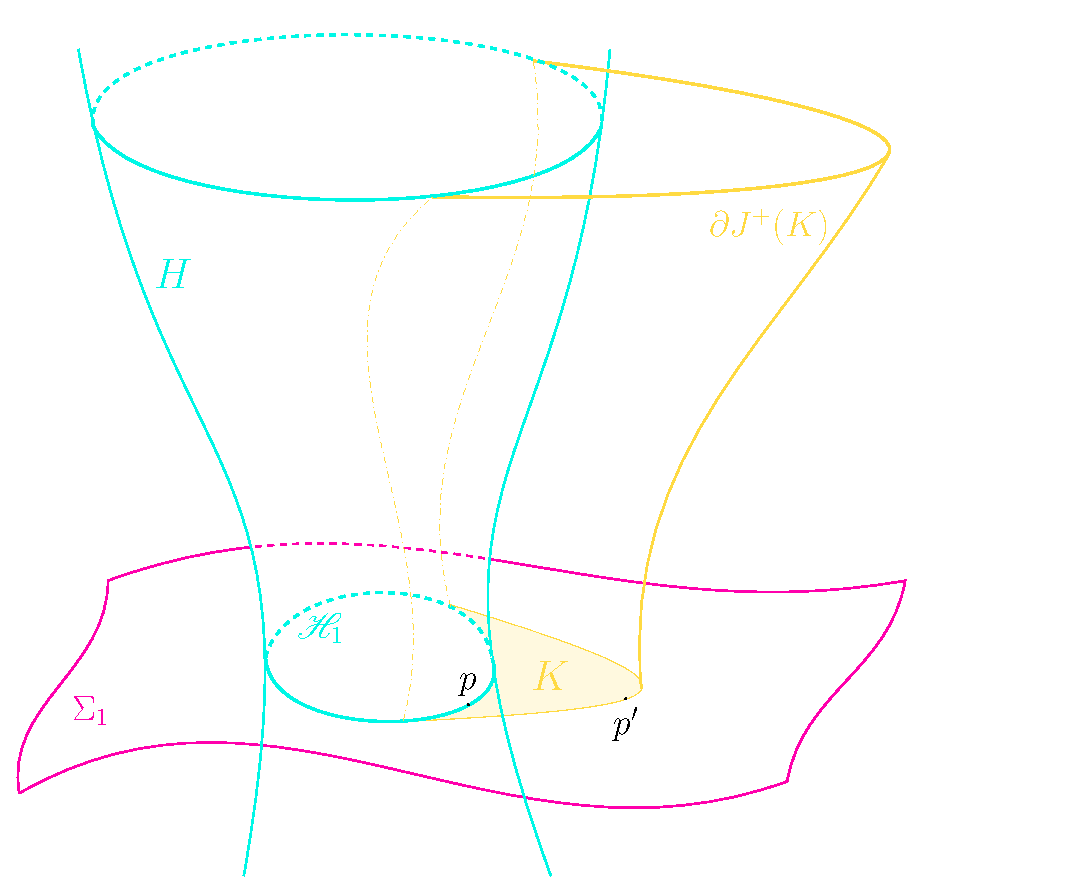
\includegraphics[scale=0.8]{Immagini/extension-area-theorem/extension-area-theorem.pdf}
		\caption[]{schematic representation about how to construct the extension of the function \(\mathrm{H}^{\mu}U_{\mu}\).}
		\label{fig:extension-area-theorem}
	\end{figure}
	\begin{SCfigure}
		\centering
		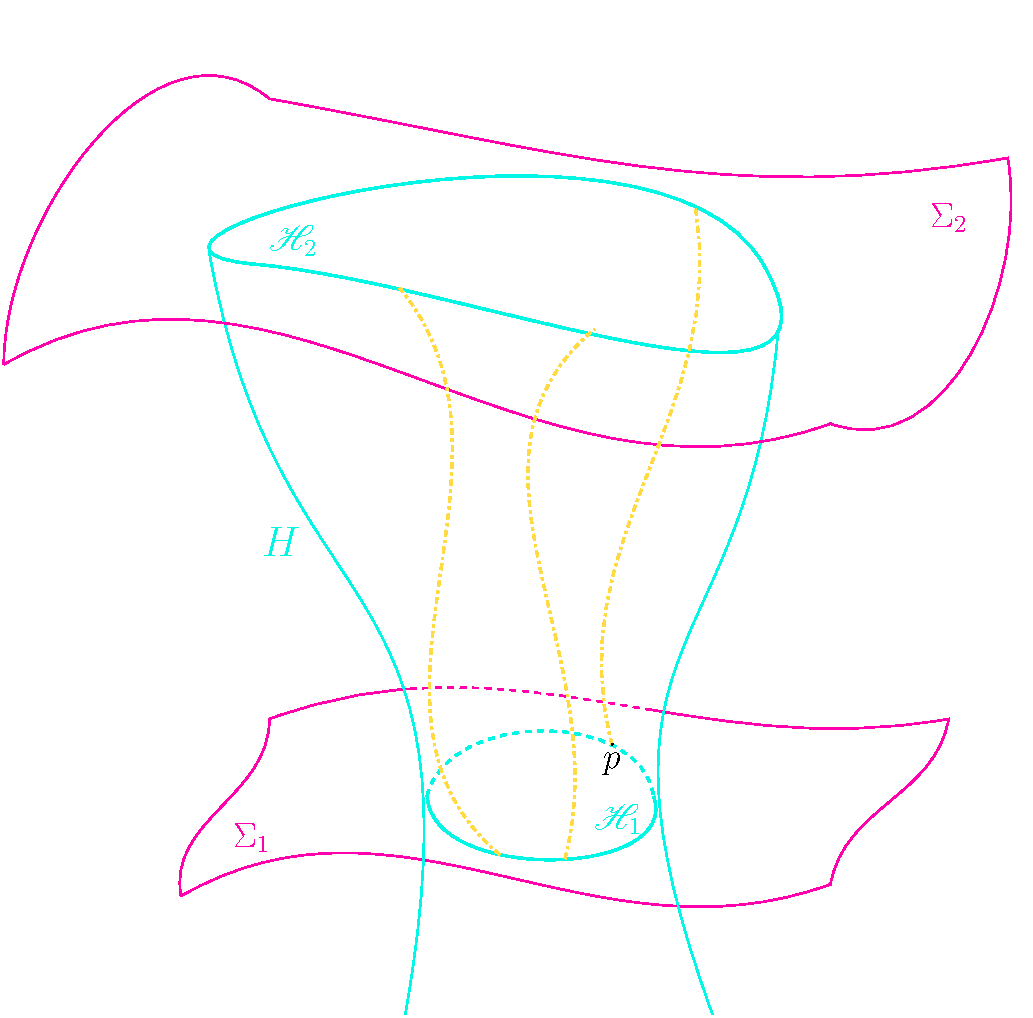
\includegraphics[scale=0.37]{Immagini/flow-generators/flow-generators.pdf}
		\caption[]{the flow along the null generators of the horizon maps \(\mathscr{H}_1\) into (a part of) \(\mathscr{H}_2\).}
		\label{fig:flow-generators}
	\end{SCfigure}
	Given that extension, for continuity it exists a neighborhood of \(p\) in which \(\mathrm{H}^{\mu}U_{\mu}(p) < 0\); we can pick a deformation \(\mathscr{H}_1\) outward on \(\Sigma_1\), to \(\mathscr{H}_1'\), such that
	\[
	\begin{cases}
	J^-(\mathscr{I}^+) \cap \mathscr{H}_1' \neq \emptyset; \\
	\mathrm{H}'^{\mu}U'_{\mu} < 0 \text{ everywhere on } 	J^-(\mathscr{I}^+) \cap \mathscr{H}_1'.
	\end{cases}
	\]
	Pick now a point \(q \in \mathscr{I}^+ \cap \partial J^+(K)\):  
	% (\VS{This exists for sth similar to 12.2.6 of Wald})
	the null geodesic generator through \(q\) will meet \(\mathscr{H}_1'\) orthogonally because of \ref{prop:global-existence} and \ref{prop:perp-critical-gamma}; however, in \(p' = \gamma \cap \mathscr{H}_1'\), \(U'_{\mu}\mathrm{H}'^{\mu} < 0\), so by proposition \ref{prop:fp-criteria} we know that a focal point to \(\mathscr{H}_1'\) must develop on \(\gamma\) before reaching \(q\). In fact, it is enough to choose \(f = 1 - \frac{\lambda}{\ell}\), with \(\lambda\) affine parameter such that:
	\[
	\begin{cases}
	\hat{\mathrm{H}}'^{\mu}U'_{\mu} = 1 \\
	\gamma(\lambda = 0) = p' \\
	\ell \ge  \frac{1}{\vert U'_{\mu}\mathrm{H}'^{\mu} \vert}
	\end{cases}
	\]
	and 
	{\small
	\[
	\int_{0}^{\ell} \big((n -2)(\nabla_{U'}f)^2 - f^2R_{\mu\nu}U'^{\mu}U'^{\nu} \big)d\lambda\le 
	\frac{n -2}{\ell} \le -(n -2) U'_{\mu} \mathrm{H}'^{\mu} =
	-(n -2) g(f^2 U', \mathrm{H}')\Big\vert_{p},
	\]}
	This is impossible, because orthogonal null generators are prompt curves, and so cannot contain any focal point (see section \ref{sec:promptness}), hence 
	\[
	\forall p \in H \quad \mathrm{H}^{\mu}U_{\mu}(p) \ge 0.
	\]
		
	To conclude, it is enough to observe that each \(p\in \mathscr{H}_1\) lies on a null generator \(\gamma\) contained in \(H\). As \(\Sigma_2\) is a Cauchy hypersurface as well, \(\gamma\) must intersect \(\Sigma_2\) in a point \(q \in \mathscr{H}_2\). Then, the flow along null generators maps \(\mathscr{H}_1\) into a portion of \(\mathscr{H}_2\) (look at figure 
	\ref{fig:flow-generators} for a pictorial representation).
	
	But we know that under deformation along the flow of a vector field, the area of a submanifold evolves as \eqref{eq:variation-area}, so:
	\begin{equation*}
		\delta_U\mathcal{A}_{\mathscr{H}_1} = \int_{\mathscr{H}_1} \mathrm{H}^{\mu}(p)U_{\mu} \ge 0
	\end{equation*}
	which is telling us that when we modify \(\mathscr{H}_1\) along the flow of the null generators the area of \(\mathscr{H}_1\) can never decrease.
\end{proof}

\begin{remark}
	As it has already been noticed in \cite[]{chrusciel2001regularity}, this statement of the area theorem is terribly vague about the proper definition of \emph{area}. The same flaw is found also in our main references \cite[]{wald2010general, hawking1973large} and in the original work on this theorem \cite[]{hawking1972black}, where it seems that picewise \(C^2\) differentiability of the horizon has been assumed. However, in \cite[]{chrusciel1998horizons} Chru\'sciel and Galloway point out that such surfaces can be pretty rough, potentially even \emph{nowhere} \(C^2\). In such cases it is not at all clear whether the notion of area or of mean normal curvature of cross-sections of the horizon would even be defined, not to mention the existence of a smooth extension of \(\mathrm{H}^{\mu}U_{\mu}\). 

	The authors in \cite[]{chrusciel2001regularity} have been able to prove a refined version of the area theorem under some slightly more restrictive assumptions, such as a notion of regularity of \(\mathscr{I}^+\), that they refer to as \(H\)-regularity. This is a very technical mathematical requirement though, which doesn't add much physical insight to our discussion, and it can be extended to all the area theorems we will prove almost straightforwardly, so for streamlining we shall not mention it anymore in the coming discussion.
\end{remark}

\subsection{The damped Averaged Null Energy Condition}
\label{subsec:dANEC-area-theorem}
In theorem \ref{th:classical-bh-area} we proved the black hole area theorem under the usual assumption of NEC. As discussed in section \ref{sec:pointwise-energy-conditions} the Null Energy Condition is violated by any sort of quantum fields (theorem \ref{th:quantum-violation-pointwise-conditions}), hence we wonder in what cases - if any - the theorem can be extended to a semiclassical regime.

One first attempt is obtained replacing the Null Energy Condition with its damped version; this result was already obtained by Lesourd in \cite{lesourd2018remark}, once again by means of the Raychaudhuri's equation, while here we would like to propose an alternative proof, in the same spirit of the one given for theorem \ref{th:classical-bh-area}.
\begin{definition}
	A spacetime satisfies the \emph{damped averaged null energy condition} (dANEC) if along each future complete null geodesic \(\gamma\), affinely parameterized by \(\lambda\), there exists a non-negative constant \(c\ge 0\) such that:
	\[
	\liminf\limits_{\Lambda\rightarrow \infty} \int_{0}^{\Lambda} e^{-c\lambda}T_{\mu\nu}U^{\mu}U^{\nu}d\lambda - \frac{c}{2} > 0
	\]
	where \(U^{\mu}\) is \(\gamma\)'s tangent field. The corresponding \emph{convergence condition} is obtained substituting \(T_{\mu\nu}U^{\mu}U^{\nu}\) with \(R_{\mu\nu}U^{\mu}U^{\nu}\), as guaranteed by Einstein equations.
\end{definition}

The statement of the theorem is the same as \ref{th:classical-bh-area}, but replacing the Null convergence condition with the dANEC equivalent; the proof is pretty similar as well but this time we will need to choose a different trial function when applying proposition \ref{prop:fp-criteria}.
\begin{proof}
	Define \(\mathscr{H}_1\), and consider \(U_{\mu}\mathrm{H}^{\mu}\) exactly as in \ref{th:classical-bh-area}. Again we want to show that it needs to be \(U_{\mu}\mathrm{H}^{\mu} > 0\) everywhere on the horizon. In order to do so, by contradiction assume there exists \(p\in \mathscr{H}_1\) for which this doesn't hold, and construct the extension \(U'_{\mu}\mathrm{H}'^{\mu}\) in a neighborhood of \(p\) in the same way as before.
	Now, pick \(f = e^{-c\frac{\lambda}{2}}\); the left hand side of \ref{eq:fp-criteria} in \(n = 4\) dimensions becomes:
	\[
	\int_{0}^{+\infty} \left((n-2)\frac{c^2}{4} e^{-c\lambda} - e^{-ct}R_{\mu\nu}U^{\mu}U^{\nu}\right)d\lambda = \frac{c}{2} - \int_{0}^{+\infty} e^{-ct}R_{\mu\nu}U^{\mu}U^{\nu}d\lambda 
	\]
	which is guaranteed to be negative by dANEC.
	Instead, \(U'_{\mu}\mathrm{H}'^{\mu} < 0 \) implies
	\[
	-(n - 2)U'_{\mu}\mathrm{H}'^{\mu} > 0.
	\]
	Hence equation \eqref{eq:fp-criteria} holds, and so a focal point must form along \(\gamma\), which is - again - absurd. 
	
	By this contradiction we have that along the null generators it must hold \(U_{\mu}\mathrm{H}^{\mu} > 0\), and the conclusion is reached exactly as in \ref{th:classical-bh-area}.
\end{proof}

From the assumption of dANEC we are still able to prove that the area cannot decrease: this is a signal that we are still working with a ``classical'' condition, in the sense that it generates a tension with the - quantum - phenomenon of black hole evaporation. We will now try to generalise the discussion, with the aim of including weaker energy conditions that could hopefully solve the tension above mentioned.


\section{A more general point of view}

The proofs of theorem \ref{th:classical-bh-area} and its dANEC version might inspire us to observe the following
\begin{lemma}
	\label{lemma:generalized-area-theorem}
	In any strongly asymptotically predictable spacetime, let \(H\) be the black hole horizon, \(U^{\mu}\) the tangent field of its null generators, and \(\mathrm{H}^{\mu}\) the mean normal curvature of \(\mathscr{H} = \Sigma \cap H\), where \(\Sigma\) is any Cauchy surface. Then it must always hold:
	\[
	U_{\mu}\mathrm{H}^{\mu} \ge -\frac{1}{n - 2} \inf_{\substack{f\in C^{\infty}_{1,0}[0, \ell]\\ \ell > 0}}J_{\ell}[f]
	\]
	where we indicated \(C^{\infty}_{1,0}[0, \ell]\) the set of smooth functions such that \(f(0) = 1\) and \(f(\ell) = 0\).
\end{lemma}

\begin{proof}
	For this proof we proceed in a similar way as in the previous section. By contradiction, suppose there exists a point \(p\) on the horizon \(H\) where:
	\[
		U_{\mu}\mathrm{H}^{\mu} < -\frac{1}{n - 2} \inf_{\substack{f\in C^{\infty}_{1,0}[0, \ell]\\ \ell > 0}}J_{\ell}[f].
	\]
	Then there exists a deformation of \(\mathscr{H}\) on the Cauchy surface \(\Sigma\) in a neighborhood of \(p\) where this inequality keeps holding everywhere, or in other words:
	\begin{equation}
		\label{eq:contradiction-generalized-area}
		\inf_{\substack{f\in C^{\infty}_{1,0}[0, \ell]\\ \ell > 0}}J_{\ell}[f] < - (n - 2)U_{\mu}\mathrm{H}^{\mu}.
	\end{equation}
	Refer again as \(K\) to the closed region between \(\mathscr{H}\) and the extension \(\mathscr{H}'\) (remember figure~\ref{fig:extension-area-theorem} for a graphical explanation).
	For the null generators of \(\partial J^+(K)\), equation~\eqref{eq:contradiction-generalized-area} implies that there exist \(\ell > 0\) and \(f\in C^{\infty}_{1,0}[0, \ell]\) so that condition~\(\eqref{eq:fp-criteria}\) is satisfied. But this leads to a contradiction in the same way as in theorem~\ref{th:classical-bh-area} because we are again in a globally hyperbolic spacetime, and null generators are not allowed to contain any focal point.

\end{proof}

Then, as before, we have that the change of the area of \(\mathscr{H}\) along the flow of null generators is controlled by
	\begin{equation*}
		\delta_U\mathcal{A}_{\mathscr{H}_1} = \int_{\mathscr{H}_1} \mathrm{H}^{\mu}(p)U_{\mu} \ge - \frac{1}{n - 2}\left(\inf_{\substack{f\in C^{\infty}_{1,0}[0, \ell]\\ \ell > 0}}J_{\ell}[f]\right)\cdot\mathcal{A}_{\mathscr{H}_1}.
	\end{equation*}
	So far we have proved that the rate of change of the area of the horizon near the reference ``time instance'' given by \(\Sigma\) cannot be lower than a certain (potentially negative) rate. 
	
\begin{remark}
	As we shall discuss in the following, the right hand side of the inequality in the thesis of lemma \ref{lemma:generalized-area-theorem} might be negative! That means that such a black hole might be able to evaporate... but we know from section \ref{sec:black-holes-evaporation} that spacetimes containing evaporating black holes are not globally hyperbolic.

	This is not a problem however: the region before the complete evaporation of the black hole remains non vicious, and Minguzzi has shown in \cite[]{minguzzi2020gravitational} that past reflectivity and this non-viciousness requirement are enough to prove Penrose's singularity theorem; in the same way our area theorem can be generalized to settings where evaporation is allowed.
\end{remark}

% In some sense this infimum is really the minimal constraint we can put on \(U_{\mu}\mathrm{H}^{\mu}\)
% \VS{Could it be equal to that by any chance? Maybe for null generators of the horizon we could say a focal point is formed at infinity, or sth like that}.
\VS{If true, I'd like to make a comment here about this bound being the strictest possible one on the rate of change of the area.}

Now, the big question we are left with is: what is the value of such infimum of \(J\)? Could it really be negative?
\noindent
This is of course a very difficult problem in general (indeed it is exactly equivalent to the original question), but there are quite a few known techniques for variational problems that can become useful.

\subsection{The first idea - a variational estimation}
\label{subsec:variational-estimation}
One possible idea - that we have already been exploiting in the specific cases of the Null energy condition and the dANEC - is really that of a variational estimation. This works as follows:
\begin{lemma}
	As soon as we can place an upper bound on \(J[f]\), holding for some class of functions \(\mathcal{A} \subset C^{\infty}_{1,0}\left([0,+\infty)\right)\), then we have an upper bound on \(\inf_{f\in C^{\infty}_{1,0}[0, \ell], \ell \ge 0}J_{\ell}[f]\), and hence a lower bound on \(U_{\mu}\mathrm{H}^{\mu}\).
\end{lemma}
	\begin{proof}
		Say that we know, from some mysterious oracle, that
		\[
		\exists f \in \mathcal{A} \quad\vert\quad J[f] \le (n-2) \cdot A.
		\]
		Then clearly
		\[
			\inf_{f\in C^{\infty}_{1,0}[0, \ell], \ell \ge 0}J_{\ell}[f] \le (n-2) \cdot A,
		\]
		and hence
		\[
			U_{\mu}\mathrm{H}^{\mu} \ge -\frac{1}{n - 2} \inf_{f\in C^{\infty}_{1,0}[0, \ell], \ell > 0}J_{\ell}[f] > - A.
		\]
	\end{proof}
	As for any variational estimation, the aim is to get a better and better approximation of the infimum by taking larger and larger sets of functions. Of course, as soon as we find any set \(\mathcal{A}\) for which the corresponding \(A\) is lower or equal than zero, we would recover the original (classical) formulation of the area theorem, and loose any interest in trying to expand further our set of functions.

	In \(J\) though, there is still hidden some metric dependence by the presence of the Ricci tensor, dependence that we would like to wash away. Here is where energy conditions shall enter and help us out again: in fact, an energy condition of the form 
	\[
	\int f^2 R_{\mu\nu}U^{\mu}U^{\nu} \ge B[f]	
	\]
	is exactly helping us in placing an upper bound on \(J\) - that doesn't depend on the metric of course, but can depend on \(f\).

	To summarise, the strategy to pursue a variational estimation of \(\inf J\) will be to pick each time:
	\begin{itemize}
		\item[\ding{99}] an energy condition of the form \(\int f^2 R_{\mu\nu}U^{\mu}U^{\nu} \ge B[f]\);
		\item[\ding{99}] a subclass of functions \(\mathcal{A}\) onto which \(J\) is easier to be ``minimized''.
	\end{itemize}
	By following this recipe we will be able to recover upper bounds on \(J\), that immediately translates to lower bounds on \(U_{\mu}\mathrm{H}^{\mu}\).

	\subsection{Classical conditions}
	An immediate observation is that, from the phenomenon of black hole evaporation, we expect the infimum of \(J[f]\) to be strictly positive.

	Instead, if we were in presence of some function \(f\) giving:
	\[
	J[f] \le 0	\iff \int_0^{\ell} f^2 R_{\mu\nu}U^{\mu}U^{\nu} \ge (n - 2)\int_0^{\ell} \vert \nabla_U f\vert^2
	\]
	then we would know that the infimum of \(J\) would have to be non positive, and so black hole evaporation would be prohibited, as it was for NEC and dANEC.

	The idea is that we would like to define an energy condition to be ``classical'' if it prohibits black hole evaporation, or in other words:
	\begin{definition}
		\label{def:classical-energy-condition}
		We say that an energy condition is \emph{classical} for a spacetime of dimension \(n\), if there exists a function in the closure of \(C_{1,0}^{\infty}\left([0, \ell]\right)\) such that
		\[
			\int_0^{+\infty} f^2 R_{\mu\nu}U^{\mu}U^{\nu} d\lambda\ge (n - 2) \int_0^{+\infty} \vert \nabla_U f\vert^2 d\lambda.	
		\]
		If the energy condition is of the form
		\[
			\int_0^{+\infty} f^2 R_{\mu\nu}U^{\mu}U^{\nu} \ge -B[f]	
		\]
		then the above becomes
		\begin{equation}
			\label{eq:definition-classical-condition}
			B[f] + (n - 2) \cdot \vert\vert \nabla_U f \vert\vert^2 \le 0.
		\end{equation}
	\end{definition}

	Accordingly, with this definition both NEC and dANEC are \emph{classical}. We explicit the examples in these two simple cases to facilitate the transition from the old proof of the area theorem to the new ideas we are exploiting.

	\textbf{Example 1 -- NEC}: As one can see from the proof of the classical black hole area theorem \ref{th:classical-bh-area}, a class of functions that works fine enough for this condition is just:
	\[
	\mathcal{A}_{NEC} = \left\{ f_{\ell}(\lambda) \coloneqq \left(1 - \frac{\lambda}{\ell}\right) \cdot \chi_{[0, \ell]}(\lambda) \vert \ell > 0 \right\},
	\]
	where with \(\chi_{[0, \ell]}\) we refer to the characteristic function of the interval \([0,\ell]\).

	Now, as for NEC \(R_{\mu\nu}U^{\mu}U^{\nu} \ge 0\) everywhere, and \(f^2 \ge 0\) as well, \(B[f] \equiv 0\). So NEC is classical according to definition \ref{def:classical-energy-condition} if we could find \(f \in \mathcal{A}_{NEC}\) such that \(\vert\vert \nabla_U f \vert\vert^2 \le 0\). But it is easy to compute that:
	\[
		\vert\vert \nabla_U f_{\ell} \vert\vert^2 = \frac{1}{\ell} \longrightarrow 0 \text{ when } \ell \rightarrow +\infty.
	\]
	\begin{remark}
		From the above procedure it is clear that whenever we choose a class of functions \(\mathcal{A}\) we can always refer to its closure \(\bar{\mathcal{A}}\) and the all procedure remains unaffected. Consequentially, limit functions can be always considered included in the sets \(\mathcal{A}\) that we pick.
	\end{remark}

	\textbf{Example 2 -- dANEC}: Similarly, looking at the proof in section \ref{subsec:dANEC-area-theorem} we can pick the set:
	\[
	\mathcal{A}_{dANEC} \coloneqq \{ f_c(\lambda) = e^{-c\frac{\lambda}{2}} \vert c >0\}.	
	\]
	Then, from the definition of dANEC we immediately recover that on \(\mathcal{A}_{dANEC}\) it holds \(B[f_c] = -\frac{c}{2}\); finally 
	\[
		\vert\vert \nabla_U f_{c} \vert\vert^2 = \frac{c^2}{4} \cdot \frac{1}{c} \implies B[f] + (n - 2) \cdot \vert\vert \nabla_U f \vert\vert^2 \equiv 0.
	\]


	\begin{corollary}
		From definition \ref{def:classical-energy-condition} it is pretty clear that any energy condition of the form
		\[
			\int_0^{+\infty} f^2 R_{\mu\nu}U^{\mu}U^{\nu} \ge -B[f]	
		\]
		where \(B[f] \le 0\) for all \(f\), then the condition needs to be classical, and therefore forbidding black hole evaporation.
	\end{corollary}
	\begin{proof}
		It is enough to use one of the sets of functions chosen in the above examples. Let's use the first one:
		\[
		\mathcal{A} \coloneqq \{f_{\ell} \quad\vert\quad \ell >0\},
		\]
		where
		\[
			f_{\ell}(\lambda) \coloneqq
			\begin{cases}
				 1 - \frac{\lambda}{\ell} \text{ for } 0 \le \lambda \le \ell, \\	
				0 \text{ for } \lambda \ge \ell.
			\end{cases}
		\]

		The norm of the first derivative has already been computed many times:
		\[
			\vert \vert \nabla_U f_{\ell} \vert\vert^2 	= \frac{1}{\ell};
		\]
		by sending \(\ell \rightarrow +\infty\), and using the hypothesis:
		\[
			B[f_{\ell}] \le 0	
		\]
		\(\eqref{eq:definition-classical-condition}\) is indeed satisfied.
	\end{proof}

\section{The Sobolev condition}
Let us finally start from an energy condition which - to the present analysis at least - leads to some more interesting consequences.
In this section we will assume the validity of a different energy condition, that uses Sobolev norms, and that's why we call it \emph{Sobolev condition}.
We have already made some comments about how we came to the choice of this conditions in section \ref{sec:sobolev-conditions}, where its definition can also found.

\subsection{Variational estimation}
\label{subsec:V-optimization}

First of all we would like to exploit this condition to obtain an estimation of \(\inf J\), using the variational procedure outlined in subsection \ref{subsec:variational-estimation}. However some care is required by the fact that the set of functions over which we need to minimize \(J\) and the one where the Sobolev condition is valid are quite different: the first one requires \(f(0) = 1\), while the second needs \(f(0) = 0\).

Closely following the analysis present in \cite[]{fewster2020new}, let us choose the set parameterized by the two real parameters \(\ell_0\) and \(\ell\):

\[
\mathcal{A}_{\beta} \coloneqq \left\{f_{\ell_0, \ell} \vert \ell > \ell_0 >0\right\} \quad\quad f_{\ell_0, \ell}(\lambda) = 
\begin{cases}
	1 \hfill \lambda\in [0, \ell_0) \\
	I(m, m; \frac{\ell - \lambda}{\ell - \ell_0}) \quad \hfill \lambda\in [\ell_0, \ell]
\end{cases}
\]
where \(I(m,m;x)\) is the regularized incomplete Beta function. This function is the unique polynomial \(p_m\) of degree \(2m - 1\) such that:
\[
p_m(0) = 0 \quad p_m(1) = 1 \quad\text{and}\quad p^{(k)}_m(0) = 0 = p^{(k)}_m(1)	\text{ for all } 1 \le k \le m - 1;
\]
it is explicitly given by \(p_m(x) = \frac{1}{B(m, m)} \int_0^x y^{m - 1}(1 - y)^{m -1} dy\), where \(B(m,m)\) is the Beta function.

In order to give an idea of what they look like, we have represented a few different such functions in figure \ref{fig:beta-functions}; finally, the values of the Sobolev norms \(A_m\) of the regularized incomplete \(m-\)Beta function, of its first derivative \(B_m\) and \(m-\)th derivative \(C_m\) are known analytically. For the sake of completeness their values are:
\[
A_m = \frac{1}{2} - \frac{(2m)!^4}{4(4m)!m!^4} \quad 
B_m= \frac{(2m-2)!^2(2m-1)!^2}{(4m-3)!(m - 1)!} \quad 
C_m = \frac{(2m-2)!(2m-1)!}{(m-1)!^2}. 
\]

\begin{figure}
	\centering
	\begin{minipage}{.45\textwidth}
	  \centering
	  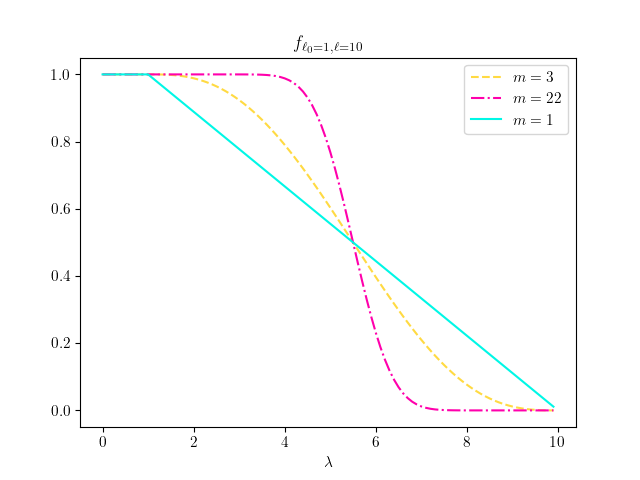
\includegraphics[width=1.1\linewidth]{Immagini/beta-functions.png}
	  \captionof{figure}{graphs of different functions in \(\mathcal{A}_{\beta}\) with \(\ell_0 = 1\), \(\ell = 10\) and \(3\) different values for \(m\). The incomplete beta function for \(m = 1\) coincides with the straight line, and becomes smoother and smoother with increasing \(m\).}
	  \label{fig:beta-functions}
	\end{minipage}
	\begin{minipage}{.45\textwidth}
	  \centering
	  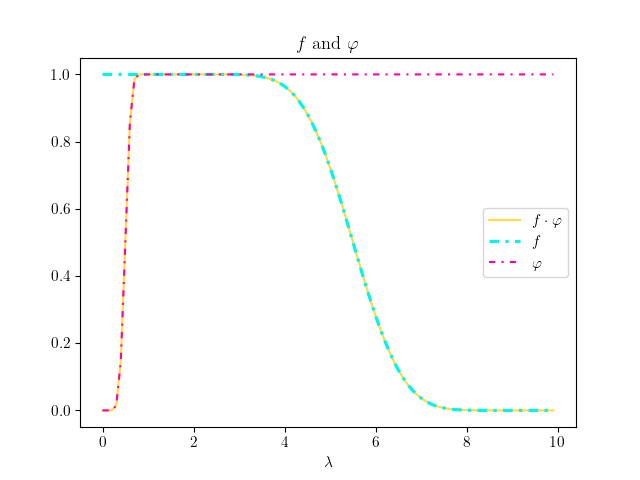
\includegraphics[width=1.1\linewidth]{Immagini/beta-functions-proof-bound.png}
	  \captionof{figure}{graphs of \(f\) and \(\varphi\) with \(\ell_0 = 1\), \(\ell=10\) and \(m = 14\), used in lemma \ref{lemma:J-sobolev-condition} to place a bound on \(J\). By taking the product of the two functions we obtain one that starts and ends at \(0\), and so can be used to apply the Sobolev energy condition.}
	  \label{fig:beta-functions-proof-bound}
	\end{minipage}
	\end{figure}

Now, assuming an additional condition on the stress energy tensor (or equivalently on the Ricci tensor), we are able to prove the following

\begin{lemma}
	\label{lemma:J-sobolev-condition}
	Assume the Sobolev condition holds, and the quantity \(\rho(\lambda) \coloneqq R_{\mu\nu}U^{\mu}U^{\nu}(\lambda) \) is lower controlled by \(\rho_0\) in \([0, \ell_0] \subseteq [0, \ell]\), or in other words
	\[
	   R_{\mu\nu}U^{\mu}U^{\nu}(\lambda) \ge \rho_0 \quad\quad \forall\lambda\in [0, \ell_0].
   \]
	Then for any \(f\in \mathcal{A}_{\beta}\) it holds:
	\begin{equation}
		\label{eq:J-sobolev-condition}
		J[f] \le (n - 2)\mathcal{V}_{\beta} \coloneqq -(1-A_m)\rho_0\ell_0 + \frac{Q_mC_m}{\ell_0^{2m-1}} + Q_0A_m\ell + \frac{(n - 2)B_m}{\ell - \ell_0} + \frac{Q_mC_m}{(\ell-\ell_0)^{2m-1}}.
	\end{equation}
\end{lemma}

\begin{proof}
	The proof of this lemma can be found in \cite{fewster2020new} as lemma \(4.1\), and it proceeds as follows. Define a piecewise smooth function \(\varphi\) on \([0,\ell]\) by:
	\[
	\varphi(\lambda) = 
	\begin{cases}
		I(m, m;\frac{\lambda}{\ell_0}) \quad \hfill \lambda \in [0, \ell_0) \\
		1 \hfill \lambda \in [\ell_0, \ell]
	\end{cases}	
	\]
	
	It's possible to see that \(\varphi f \in W_0^m([0,\ell])\), so writing \(f^2 = (\varphi f)^2 + (1 - \varphi^2)\) we have:
	\begin{align*}
		\int_0^{\ell} f(\lambda)^2\rho(\lambda) &\ge \int_0^{\ell} (1 - \varphi(\lambda)^2)\rho(\lambda)d\lambda - Q_m(\gamma) \vert\vert (\varphi f)^{(m)}\vert\vert^2 - Q_0(\gamma) \vert\vert \varphi f\vert\vert^2 \\
		&\ge  \rho_0\int_0^{\ell} (1 - \varphi(\lambda)^2)d\lambda - Q_m(\gamma) \vert\vert (\varphi f)^{(m)}\vert\vert^2 - Q_0(\gamma) \vert\vert \varphi f\vert\vert^2.
	\end{align*}

	Moreover, the norms of the functions can be analytically computed for the specific choices that we made:
	\[
		\vert\vert \varphi f\vert\vert^2 = A_m\ell_0 + A_m(\ell - \ell_0)\quad
		\vert\vert (\varphi f)^{(m)}\vert\vert^2 = \frac{C_m}{\ell_0^{2m - 1}} + \frac{C_m}{(\ell - \ell_0)^{2m - 1}}
		\quad
		\vert\vert f'\vert\vert^2 = \frac{B_m}{\ell - \ell_0}
	\]
	Thus,
	\[
		J[f] \le \frac{(n - 2)B_m}{\ell - \ell_0} + \frac{Q_mC_m}{\ell_0^{2m - 1}} + \frac{Q_mC_m}{(\ell - \ell_0)^{2m - 1}} + Q_0A_m\ell - \rho_0\ell_0(1 - A_m) \coloneqq (n-2)\mathcal{V}_{\beta},
	\]
	and the estimate is complete.
\end{proof}

\begin{SCfigure}
	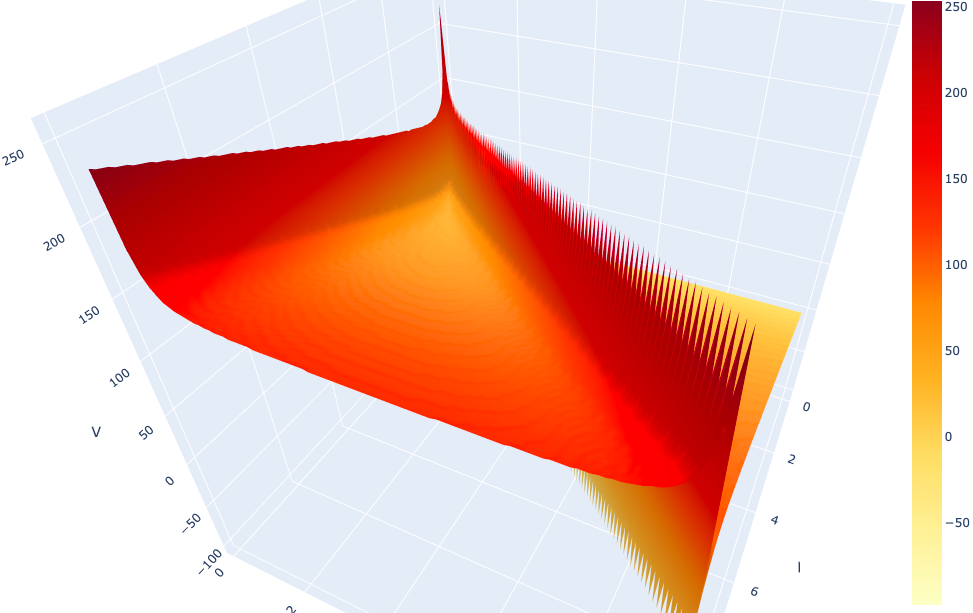
\includegraphics[scale=0.28]{Immagini/V-beta.png}
	\caption[]{plot of \(\mathcal{V}_{\beta}(\ell_0, \ell)\) (\(\hat{z}\) axis). On the right it appears part of the \(\ell\) axis, while the hidden one corresponds to \(\ell_0\). The color-scale should help to spot out the minimum of the visualized sheet.}
	\label{fig:V-beta}
\end{SCfigure}

Now that for each function \(f_{\ell_0, \ell} \in \mathcal{A}_{\beta}\) we have an estimate for \(J\left[f_{\ell_0, \ell}\right] \le (n-2)\mathcal{V}_{\beta}(\ell_0, \ell)\), we can finally pursue the variational strategy: we need to minimize \(\mathcal{V}_{\beta}(\ell_0, \ell)\) on \(\ell \ge \ell_0\). In order to do so we will first minimize along \(\ell\), keeping \(\ell_0\) fixed, and then proceed to a second minimization over this last parameter.

The first optimization has been already performed in \cite{fewster2020new}, even if in their computation they neglect some terms that instead will be relevant for us, because of the different regime of approximation that we will need to set. Let then us do that, with the additional restriction of \(m = 1\): in the following this request will always be fulfilled, so this is the most general we need to be, but this procedure could be generalized to arbitrary \(m\) at the price of solving a higher order algebraic equation.

\begin{prop}
    For \(m = 1\), the bound optimized on \(\ell \ge \ell_0\) is
    \[
      (n-2)\mathcal{V}_{\beta}(\ell_0) = (A_1 - 1)\rho_0\ell_0 + \frac{Q_1C_1}{\ell_0} + 2 \sqrt{(n - 2)A_1B_1Q_0}   
    \]
    and is obtained for:
    \[
    \tilde{\ell} = \ell_0\left(1 + \sqrt{\frac{(n - 2) B_1}{A_1 Q_0\ell_0^2}}\right)    
    \]
\end{prop}

\begin{proof}
    The proof is very similar to the one given in \cite{fewster2020new}, but we have to pay attention to keep all the terms relevant for us.
	\noindent
    Set \(\ell = \ell_0\left(1 + B_1\mu\right)\), so that the constraint \(\ell\ge\ell_0\) becomes simply \(\mu \ge 0\).
    % The interesting case presents when \(\mu \ge 1\), for which \(\frac{1}{\mu^{2m - 1}} \le \frac{1}{\mu} \) (in particular in subsection \ref{subsec:non-min-EKG-theory} we will focus on the \(m = 1\) case, where the equality holds). 
	The expression in \(\eqref{eq:J-sobolev-condition}\) reduces to:
    \begin{align*}
        \mathcal{V}(\ell, \ell_0) &= E + F\mu + \frac{G}{\mu} \\
        E &= (A_m - 1)\rho_0\ell_0 + Q_0A_m\ell_0 + \frac{Q_mC_m}{\ell_0}\\
        F &= Q_0A_mB_m\ell_0 \\
        G &= \frac{n- 2}{\ell_0} + \frac{Q_mC_m}{B_m\ell_0}
    \end{align*}
    Imposing the first derivative w.r.t \(\ell\) of \(\mathcal{V}_{\beta}\) to be zero, it is easy to obtain:
    \[
    \tilde{\mu} = \sqrt{\frac{G}{F}} =  \sqrt{\frac{n - 2}{A_1B_1Q_0\ell_0^2}}.
    \]
	where we neglected the second term of \(G\) under the assumption \(Q_1 \ll 1\); in the following we will see that \(Q_1 \sim \left(\frac{T}{T_{Pl}}\right)^2\), so assuming \(Q_1 \ll 1\) corresponds to be in the temperature regime where \(\left(\frac{T}{T_{Pl}}\right)^2 \ll 1\), which is not particularly restrictive as also the analysis of black hole evaporation is performed under the same assumption.
\end{proof}

Now we reduced to a bound that only depends on \(\ell_0\) (and some other global feature of the system, summarized within \(Q_0\) and \(Q_m\)); in light of the variational strategy, let us finally proceed to the last minimization and find the optimal value for \(\ell_0\)\footnote{Actually, there were several possibilities that could have been explored with the aim of providing an estimate for \(\ell_0\). The first idea was to pick some constant \(\ell_0\) (which is what has been done in \cite{fewster2020new}), fixed to be some relevant physical quantity, but we haven't been able to formulate one particularly convincing. Besides, requiring \(\ell_0\) to be constant in a background that will be dynamic didn't seem particularly reasonable after all, so we decided to minimize \(\mathcal{V}_{\beta}\) - and finally outlined the variational procedure.}. 

\begin{prop}
	Assuming \(\rho_0 < 0\) the optimal bound, minimized along \(\ell_0\), is:

	\begin{equation}
		\label{eq:minimized-V-beta}
		\mathcal{V}_{\beta} = \frac{5}{6}\sqrt{\frac{3}{2}Q_1 \vert\rho_0\vert} + 2 \sqrt{(n - 2)A_1B_1Q_0}
	\end{equation}

	corresponding to \(\tilde{\ell}_0^2 = - \frac{3Q_1}{2\rho_0}\)
\end{prop}
\begin{proof}
	The computation is very similar to the preceding one, as in particular the shape of the function to be minimized is exactly the same.
\end{proof}

Lemma \ref{lemma:generalized-area-theorem} can now immediately tell us that, in an asymptotically flat spacetime, wherever on the null generators of the black horizon the Sobolev energy condition holds and \(R_{\mu\nu}U^{\mu}U^{\nu} \ge \rho_0\), then the instantaneous rate of expansion of the cross-sectional area is constrained by
\begin{equation}
	\label{eq:area-sobolev-condition}
	U_{\mu}\mathrm{H}^{\mu} \ge - \mathcal{V}_{\beta} \implies \delta_U\mathcal{A}_{\mathscr{H}_1} = \int_{\mathscr{H}_1} \mathrm{H}^{\mu}(p)U_{\mu} \ge - \mathcal{V}_{\beta}\cdot\mathcal{A}_{\mathscr{H}_1},
\end{equation}
where, again, the implication is possible thanks to lemma \ref{lemma:variation-area}. We will argue later that the assumption \(\rho(\lambda) \ge \rho_0\) in a small interval of the affine parameter is well motivated, and we will find \(\rho_0 < 0\), so \eqref{eq:minimized-V-beta} is well defined, and \(\mathcal{V}_{\beta} >0\). This means we have proved that the rate of change of the area of the horizon near the reference ``time instance'' given by \(\Sigma_1\) cannot be lower than a certain - negative - rate!

Equation \eqref{eq:area-sobolev-condition} can then truly claim to be a first non trivial generalization of Hawking's area theorem: it is still placing a lower bound on the rate of evolution of the area, but, as the bound is negative this time, it can - in principle - resolve the tension with the quantum phenomenon of evaporation, now potentially allowed.
	
Notice however that, conversely to the original theorem, we have only constrained the \emph{instantaneous} rate of change. Here it is not possible to directly set bounds on the average rate of evolution between \(2\) arbitrarily far Cauchy surfaces \(\Sigma_1\) and \(\Sigma_2\), as for that we would need to assume the Sobolev condition and the pointwise restriction \(\rho \ge \rho_0\) in the all region in between \(\Sigma_1\) and \(\Sigma_2\), which would mean a significant weakening of our result.

\subsection{The second idea -- a differential equation}
\label{subsec:E-L-optimization}
A potential weakness of the variational method is that, if the set \(\mathcal{A}\) onto which the optimization is performed is not chosen with enough care, its extremum may still lay very far from \(\inf J\). Referring to the above subsection \ref{subsec:V-optimization}, it might happen that even if \(\mathcal{V}_{\beta} > 0\), the actual \(\inf_{f\in C^{\infty}_{1,0}[0, \ell], \ell \ge 0}J\) is negative, and hence evaporation is not allowed.

Such question can only be completely resolved by finding the true infimum, or a set \(\mathcal{A}\) where the minimum is negative. We are not able to do that unfortunately, but we can look at our results and see if anything stands out. 

It may attract our attention the curious feature that the minimum of \(\mathcal{V}_{\beta}\) lays at finite \(\ell\): a simple heuristic argument instead suggests that a priori we should expect it to be at \(\ell \rightarrow +\infty\).

\(\ell\) is nothing but the maximum length of the support of the function \(f\). Ideally, in order to minimize \(J[f]\), we should expect \(f\) to be non zero wherever \(R_{\mu\nu}U^{\mu}U^{\nu}\) is positive, and null (or almost null) wherever \(R_{\mu\nu}U^{\mu}U^{\nu} < 0\). By cutting out the possibility of exploring for \(\lambda \ge \ell\) we might just miss out some regions where \(\rho(\lambda)\) is positive again. 

\noindent
Analogously, when energy conditions of the form above mentioned come into force, instead of optimizing \(J\) we try to minimize \(\vert\vert \nabla_U f\vert\vert^2 + B[f]\), and again - as \(f\) is required to go from \(1\) at \(\lambda = 0\) to \(0\) at \(\lambda = \ell\) - by pushing \(\ell\) as far away as possible we would suppress the norms of all the derivative of \(f\).

We may then wonder how reasonable is the result we have obtained in \eqref{eq:area-sobolev-condition}; to test it we developed an alternative method, that is a combination of an Euler-Lagrange approach and the variational method. Suppose again to start from an energy condition of the form
	\[
		\int_0^{\ell} f^2 R_{\mu\nu}U^{\mu}U^{\nu} \ge -B[f] \implies J[f] \le \vert\vert \nabla_U f\vert\vert^2 + B[f]
	\]
and then, instead of choosing any set \(\mathcal{A}\), we write an Euler-Lagrange equation - that doesn't depend on the metric - to minimize 
	\[
	\vert\vert \nabla_U f\vert\vert^2 + B[f] \quad\text{ with }\quad f(0) = 1 \quad \quad f(\ell) = 0.	
	\]

Even if this is the main idea, we can only apply the Sobolev energy condition to functions that have Dirichlet boundary conditions; with some work it is possible to get to a differential equation also in the general case, but one that is too hard to be solved - at least for us.
By reducing to the set of functions (here's why we say that this method is partially a variational estimation again)
\[
\mathcal{A}_{E.L.} \coloneqq \{f \quad \vert \quad \exists \ell_0 > 0 \text{ s.t. } f(\lambda \le \ell_0) \equiv 1\} \supset \mathcal{A}_{\beta}
\]
the problem becomes doable, and we obtain:
\begin{equation}
	\label{eq:V-euler-lagrange}
	\mathcal{V}_{E.L.}(\ell_0, \ell) = \sqrt{Q_0(n - 2 + Q_1)}\coth\left[\Omega_1(\ell- \ell_0)\right] + \sqrt{Q_0Q_1}\coth\left[\Omega_2\ell_0\right] + \vert \rho_0\vert\ell_0
\end{equation}
where
\[
\Omega_1^2 = \frac{Q_0}{n - 2 + Q_1} \quad \quad  \Omega_2^2 = \frac{Q_0}{Q_1}.
\]

All the main ideas behind this procedure have already been explained with enough detail in the present section or in \ref{subsec:V-optimization}, so we defer the computation that proves equation \eqref{eq:V-euler-lagrange} to appendix \ref{app:V-E-L-optimization}.

\begin{SCfigure}
	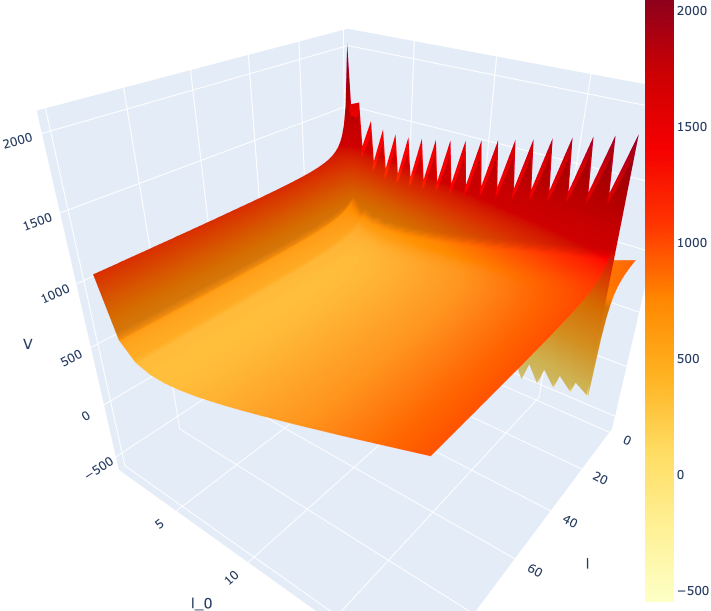
\includegraphics[scale=0.3]{Immagini/V-E-L.png}
	\caption[]{Plot of \(\mathcal{V}_{E.L.}(\ell_0, \ell)\); this plot can be directly compared to the one in figure \ref{fig:V-beta} and again it stands out that this time the minimum will lay at large \(\ell\).}
	\label{fig:V-E-L}
\end{SCfigure}

Once more, we minimize \(\mathcal{V}_{E.L.}(\ell_0, \ell)\) on \(\ell \ge \ell_0\) in order to recover the best possible bound on \(\inf J\). We immediately see that this time the minimum is found for \(\ell \rightarrow +\infty\): the only \(\ell-\)dependence is in \(\coth\left[\Omega_1(\ell- \ell_0)\right]\), which is monotonically descending towards \(1^+\).

For \(\ell_0\) instead, the minimum is found at \(\tilde{\ell}_0 = \sqrt{\frac{Q_1}{Q_0}}\sinh^{-1}\left(\sqrt{\frac{Q_0}{\vert\rho_0\vert}}\right)\), so that in the end we have
{\small
\begin{equation}
	\label{eq:minimized-V-E-L}
	U_{\mu}\mathrm{H}^{\mu} \ge - \frac{1}{n - 2}\mathcal{V}_{E.L.} =  \frac{1}{n - 2} \left\{ \sqrt{Q_0(n - 2 + Q_1)} + \sqrt{Q_1(Q_0 + \vert\rho_0\vert)} + \frac{3}{2}\sqrt{Q_1\vert\rho_0\vert} \right\}.
\end{equation}}

Notice that, even if \(\mathcal{A}_{E.L.}\) is a much larger set than \(\mathcal{A}_{\beta}\), the result in \eqref{eq:minimized-V-E-L} is very similar to the one in \eqref{eq:minimized-V-beta}; indeed only some coefficients are changed, but the qualitative behaviour is always the same, and in particular \(\mathcal{V}_{E.L.}\) stays negative.

\section{Comparison with the evaporation rate}
\label{sec:physical-interpretation-V}

Coherently, with the weakening of the energy condition we have obtained a weaker constraint: but what is the real physical impact of the new hypothesis we have taken?

As extensively argued above, \(\mathcal{V}\) represents the bound on the instantaneous rate of change of the area of the black hole horizon. In order to understand how reasonable it is the expression we have obtained, we would need to compare it to some relevant physical quantity; in this scenario we are lucky enough to have a particular appealing one: the rate of black hole evaporation.

With that in mind, we need to translate the mathematical expression of \(\mathcal{V}\) given in \(\eqref{eq:minimized-V-E-L}\) into a function of physical quantities only; once again we will let us be inspired by the work in section \(5.2\) of \cite{fewster2020new}, where Fewster and Kontou computed their bound in the specific framework of a non-minimally coupled classical Einstein-Klein Gordon theory.

They needed such a computation to test the hypothesis of some weakened singularity theorems within astrophysical scenarios; here instead we would like to analyze the evaporation of black holes, and so we will need a different regime of approximations.

\subsection{The non-minimally coupled Einstein Klein Gordon Theory}
\label{subsec:non-min-EKG-theory}
First of all let's try to compute some reasonable physical estimates of the coefficient \(Q_0\) and \(Q_m\). In order to do so we need to pick a specific field theory, and we will adopt a semiclassical gravity point of view, so quantum fields within a classical background geometry, where backreaction corrections are assumed small - and thus neglected.

Our choice happens to land on non-minimally coupled scalar fields: this is the typical classical field theory violating NEC, and thus the original black hole area theorem doesn't apply. They are scalar fields described by the Lagrangian density
\[
\mathcal{L}[\phi] = -\frac{1}{2}\left[\nabla_{\mu}\phi\nabla^{\mu}\phi   - (m^2 - \xi R)\phi^2\right]
\]
The corresponding stress-energy tensor is:
\begin{equation}
    T_{\mu\nu} = \nabla_{\mu}\phi\nabla_{\nu}\phi - \frac{1}{2}g_{\mu\nu}\left[\nabla_{\rho}\phi\nabla^{\rho}\phi - m^2\phi^2\right] + \xi\left(g_{\mu\nu}\square_g - \nabla_{\mu}\nabla_{\nu} + G_{\mu\nu}\right)\phi^2
\end{equation}
% La derivazione di https://alves-nickolas.github.io/pdf/Stress_Energy_Momentum_Tensor_for_a_Scalar_Field.pdf mi e' piaciuta
The conformal coupling is \(\xi_c = \frac{1}{4}\frac{n - 2}{n - 1}\), and we will only consider \(\xi\in [0,\xi_c]\);
now the following observation comes along.

\begin{prop}
    It is physically reasonable to impose that \(8\pi\xi\phi^2 < 1\).
\end{prop}

\begin{proof}
    The argument can be found in \cite{kontou2020energy} and starts by rearranging Einstein equations in the following form:
    \[
      \frac{1 - 8\pi\xi\phi^2}{8\pi}G_{\mu\nu} =  \underbrace{\nabla_{\mu}\phi\nabla_{\nu}\phi - \frac{1}{2}g_{\mu\nu}\left[\nabla_{\rho}\phi\nabla^{\rho}\phi - m^2\phi^2\right] - \xi\left(g_{\mu\nu}\square_g - \nabla_{\mu}\phi\nabla_{\nu}\right)\phi^2}_{T^{eff}_{\mu\nu}}.
    \]
    Notice that - for \(\xi > 0\) - the coefficient in front of \(G_{\mu\nu}\) vanishes for \(8\pi\xi\phi^2 = 1\); for such values of the field \(\phi\) the order of Einstein equations reduces, and so the initial value problem becomes ill-defined.

    When \(8\pi\xi\phi^2 \neq 1\) instead, Einstein equations become:

    \[
        G_{\mu\nu} = \frac{8\pi}{1 - 8\pi\xi\phi^2}T^{eff}_{\mu\nu},
    \]
    and so we can see that for \(8\pi\xi\phi^2 > 1\) we would have a negative ``effective Newton's constant''. 

    This is not a definitive proof that non-minimally coupled fields cannot access such high values (called \emph{trans-Planckian}), but it is more a motivation about why it seems reasonable to assume that bound. 
\end{proof}

From here onward we will assume that non-minimally coupled scalar fields will always obey the bound:
\[
\phi^2 < \frac{1}{8\pi\xi}.    
\]
Moreover we shall only consider \emph{massless} scalar fields; given that, it was shown in \cite{fewster2011singularity} and \cite{brown2018singularity} that the Ricci tensor contraction is bounded by a Sobolev-like energy condition.

\begin{prop}
    In the context of a massless non-minimally coupled Einstein-Klein Gordon field theory, the integral of the contraction of the Ricci tensor along any causal geodesic, weighted with any compactly supported real valued \(-\frac{1}{2}\)-density \(f\), is bounded by:

    \begin{equation}
        \int_{\gamma}f^2 R_{\mu\nu}U^{\mu}U^{\nu} \ge -Q\left(\vert\vert\nabla_U f \vert\vert^2 + \tilde{Q}^2 \vert\vert f\vert\vert^2\right).
    \end{equation}
    where 
    \[
    Q = \frac{32\pi\xi\phi_{max^2}}{1 - 8\pi\xi\phi_{max}
    ^2}
    \quad\quad
    \tilde{Q} = \frac{8\pi\xi\phi_{max}}{1 - 8\pi\xi\phi_{max}
    ^2}\sup_{\gamma}\vert \nabla_U\phi\vert.
    \]
\end{prop}

The proof of is lengthy and not particularly interesting for the scope of this thesis, so we defer it to appendix \ref{app:proof-EKG-bound}.

We have indeed found an energy condition of the form \(\eqref{eq:Sobolev-condition}\) with 
\[
m = 1 \quad\quad Q_0 = Q\cdot\tilde{Q}^2 \quad\quad Q_1 = Q 
\]

\subsection{The Kubo-Martin-Schwinger state}

In order to finally convert \(Q_0\) and \(Q_1\), we need to compute \(\phi_{max}\) and \(\sup_{\gamma}\vert \nabla_U\phi\vert\) in terms of some physical quantities; in principle the field values may be not bounded, but here we only aim at estimating what a reasonable value for \(\mathcal{V}\) would be.
Physically, it makes sense that the value of \(\phi_{max}\) is connected to some sort of background temperature, and we expect the higher \(T\) is, the higher values \(\phi\) might reach.

In order to establish this connection we now change setting, and consider a \emph{quantum} field theory with a minimally coupled massless scalar field in a Minkowski background metric; we aim at computing the Wick square of our field averaged in a thermal state of temperature \(T\). As choice of thermal state, we pick the Kubo-Martin-Schwinger (KMS) state with temperature \(T\), as in section \(5.2\) of \cite{fewster2020new}, where we can compute the desired quantity in a way analogous to what has been done in the final appendix of \cite{brown2018singularity}.

% \begin{definition}
%     The KMS state is defined as \dots
%     %todo: studiare
% \end{definition}

\begin{remark}
	The KMS state is a \emph{thermal equilibrium} state. This means we must be working with quasi-static black holes, which are evaporating so slowly that can be thought always in nearly thermal equilibrium with the background. This approximation should be well verified because, once again, it coincides with the temperature regime \(\frac{T}{T_{Pl}}\ll 1\).
\end{remark}

\begin{prop}
	\label{prop:wick-squares-KMS}
    The Wick square of the massless field, in a KMS thermal state of temperature \(T\), within a \(n\)-dimensional Minkowski spacetime, is given by:
    \begin{align*}
         \langle \colon \phi^2 \colon\rangle_T &= \frac{T^{n - 2}}{2^{n - 2}\pi^{\frac{n - 1}{2}}}\frac{\Gamma(n - 2)}{\Gamma\left(\frac{n - 1}{2}\right)}\zeta(n - 2) \\
        \langle \colon (\nabla_U\phi)^2 \colon\rangle_T &= \frac{nT^n}{2^{n - 1}\pi^{\frac{n - 1}{2}}} \frac{\Gamma(n)}{\Gamma\left(\frac{n + 1}{2}\right)} \zeta(n)
    \end{align*}

\end{prop}
    
\begin{proof}
    Given \(\beta = \frac{1}{k_BT}\) the \(2\)-point function of the state is:
	\[
	W^{(2)}_T(x, x') = \int \frac{d^{n - 1}\mathbf{k}}{(2\pi)^{n - 1}}\frac{1}{2k^0(\mathbf{k})} \left(\frac{e^{-ik^{\mu}(x_{\mu} - x'_{\mu})}}{1 - e^{-\beta k^0(\mathbf{k})}} + \frac{e^{ik^{\mu}(x_{\mu} - x'_{\mu})}}{e^{\beta k^0(\mathbf{k})} - 1}\right). 
	\]

	As we are dealing with a massless scalar field, the dispersion relation is \(k^0(\mathbf{k}) = \vert \mathbf{k}\vert\) (the field is on-shell).

	For the ground state \(2\)-point function we need to take the limit \(T\rightarrow 0\), or \(\beta\rightarrow +\infty\), and obtain
	\[
	W^{(2)}_0(x, x') = \int \frac{d^{n - 1}\mathbf{k}}{(2\pi)^{n - 1}}\frac{1}{2k^0(\mathbf{k})} e^{-ik^{\mu}(x_{\mu} - x'_{\mu})}. 
	\]
	The Wick square is defined to be:
	\[
		\langle \colon \phi^2 \colon\rangle_T = \lim_{x'\rightarrow x} \left[W^{(2)}_T(x, x') - W^{(2)}_0(x, x')\right]
	\]
	The above expression can be simply worked out to be:
	\begin{align*}
		\langle \colon \phi^2 \colon\rangle_T &= \underbrace{\frac{2\pi^{\frac{n-1}{2}}}{\Gamma(\frac{n - 1}{2})}}_{\Omega_{n - 2}}\frac{1}{(2\pi)^{n - 1}}\frac{1}{\beta^{n - 2}}\int_0^{+\infty}dx \frac{x^{n - 3}}{e^x - 1} =\\
		&= \frac{T^{n - 2}}{2^{n - 2}\pi^{\frac{n - 1}{2}}}\frac{\Gamma(n - 2)}{\Gamma\left(\frac{n - 1}{2}\right)}\zeta(n - 2)
	\end{align*}
	The second inequality can be worked out in a similar way, being careful that this time there is an angular dependance because of the additional factor \((k_{\mu}U^{\mu})^2\), originated by the \(U\)-derivatives. This factor adds a \(k^2\) power to the radial part of the integral, and an angular factor:
	\[
	\int_0^{\pi} \sin\theta^{n - 3} (1 - \cos\theta)^2 d\theta = \frac{n\sqrt{\pi}}{2}\frac{\Gamma\left(\frac{n - 2}{2}\right)}{\Gamma\left(\frac{n + 1}{2}\right)}.
	\]
	So the final result becomes:
	\begin{align*}
		\langle \colon (\nabla_U\phi)^2 \colon\rangle_T &= 
		\underbrace{\frac{2\pi^{\frac{n-2}{2}}}{\Gamma(\frac{n - 2}{2})}}_{\Omega_{n - 3}} \cdot \frac{n\sqrt{\pi}}{2}\frac{\Gamma\left(\frac{n - 2}{2}\right)}{\Gamma\left(\frac{n + 1}{2}\right)} \cdot \frac{1}{(2\pi)^{n - 1}}\frac{1}{\beta^{n}}\int_0^{+\infty}dx \frac{x^{n - 1}}{e^x - 1} = \\
		&= \frac{nT^n}{2^{n - 1}\pi^{\frac{n - 1}{2}}} \frac{\Gamma(n)}{\Gamma\left(\frac{n + 1}{2}\right)} \zeta(n).
	\end{align*}
\end{proof}

At last we estimate the maximum values of the \emph{classical} E-KG field and its derivative by the ansatz 
\begin{align*}
	\phi_{\max}^2 &\simeq \langle \colon \phi^2 \colon\rangle_T,\\
	\sup_{\gamma}\vert \nabla_U\phi\vert &\simeq \langle \colon (\nabla_U\phi)^2 \colon\rangle_T.
\end{align*}
Restoring units and reducing to \(n = 4\) spacetime dimensions, we eventually obtain:
\begin{align}
	\label{eq:KMS_Q_1}
    Q_1 &= \underbrace{\frac{16\pi\xi}{3}}_{\alpha} \left(\frac{T}{T_{Pl}}\right)^2,\\
    Q_0 &= \underbrace{\frac{32\pi^6\xi^3}{405}}_{\gamma}\left(\frac{k_B}{\hbar}\right)^2 \frac{T^8}{T_{Pl}^6}.
\end{align}

Again, this is of course not a rigorous computation of the coefficients, but it is a meaningful approximation pursued in an instructive toy-model, that can give us some encouraging insights on the underlying complicated physics.

For the purpose of the following analysis we will identify \(T\) with the Hawking temperature of the black hole \(\eqref{eq:hawking-temperature}\):
\[
T_H = \frac{\hbar c^3}{8\pi Gk_B}\frac{1}{M}    
\]
    
\begin{remark}
	The toy model we relied on in this section has, of course, many limitations. One we have tried to resolve is due to the definition of the \(2\)-point function of KMS states - used to prove proposition \ref{prop:wick-squares-KMS} - only in Minkowski spacetime. The proper state to describe a black hole in thermal equilibrium within an underlying Schwarzschild geometry is the Hartle-Hawking state \cite[]{hartle1993path}. This state has been proved to be equivalent to the double KMS state with temperature equal to Hawking temperature, first in \cite[]{jacobson1994note, sanders2015construction} (with the path integral formulation), and lately in \cite[]{higuchi2022hartle} by means of the Schwinger-Keldysh operator formalism. Unfortunately the \(2\) point function is a little more complicated than the one in the flat space case:
	\[
	W_{HH}(x, x') = \int_{0}^{+\infty} \frac{d\omega}{2\omega} \sum_{\sigma}\phi_{\omega\sigma}(x)\phi_{\omega\sigma}(x')\left(\frac{e^{-i\omega(t - t')}}{1 - e^{-\beta \omega}} + \frac{e^{i\omega(t - t')}}{e^{\beta \omega} - 1}\right),
	\]
	where \(\{\phi_{\omega\sigma}(x)\}\) are a basis of the set of solutions to the equations of motion. In flat spacetime the factor \(\sum_{\sigma}\phi_{\omega\sigma}(x)\phi_{\omega\sigma}(x')\) simply reduces to 
	\[
		\int_{\vert k \vert = \omega}	\frac{dk^{n - 1}}{(2\pi)^{n - 1}} e^{-i\vec{k}\cdot \vec{x}},
	\]
	but as for now we didn't manage to work it out in the Schwarzschild case. Working out the additional temperature dependence - if any - given by such factor would be enough to properly generalize our method to Schwarzschild.
\end{remark}

\subsection{Limited violations}
\label{subsec:rho-0-estimation}

In order to estimate the value of the functional \(J[f]\) we required 
\[
	\rho (\lambda)\coloneqq R_{\mu\nu}U^{\mu}U^{\nu}\ge -\vert\rho_0\vert
\] 
for \(\lambda\in [0, \ell_0]\); this is again a pointwise requirement, but notice that, as the lower bound is negative, it is not ruled out by the argument in \ref{th:quantum-violation-pointwise-conditions}.

It has been for long debated whether such contractions of the stress energy tensor should be finite or not; in literature there can be found arguments for both sides, and indeed a lot of attention must be payed to what contraction exactly is going to be computed. The presence of a coordinate singularity, and the lack of an analytical expression for the \(4\)-dimensional stress-tensor in the Unruh or Hartle-Hawking state complicate the matter, but we will try to argue that - as the one on the horizon is \emph{just} a coordinate singularity - the contraction of \(T_{\mu\nu}\) with the tangent field of the null generators shall be always finite.

Let us again work within the framework of non-minimally coupled scalar fields, with \(\xi\in[0,\xi_c]\); developing a general treatment is very difficult because of the features mentioned above, but at the two extremities of this interval  a few observation can be inferred.

For \(\xi = 0\) the field becomes minimally coupled; the classical minimally coupled Klein-Gordon field actually obeys the Null Energy condition, but this doesn't mean that the quantized field shouldn't bear any surprise.
Indeed, in \cite{levi2016versatile} Levi and Ori have been able to overcome many of the complications for the computation of a renormalized stress tensor in the Unruh vacuum, and managed to run some numerical simulations to estimate \(\rho\) in the outer proximity of the horizon, within a background Schwarzschild metric. 
Recasted with our convention (for us their \(a\) needs to be \(1\)), their result is 
\begin{equation}
	\label{eq:rho-Levi-Ori}
	\rho \simeq -2.7\cdot 10^{-7} \frac{\hbar}{M^{4}} 
\end{equation}
(where \(M\) is the mass of the black hole). This supports the legitimacy of our additional assumption, at least for large enough black holes, and suggests that such a condition might be commonly satisfied even with a rather small value of \(\vert\rho_0\vert\). The most important features of Levi and Ori's result~\eqref{eq:rho-Levi-Ori} are the negative sign and the \(M^{-4}\) dependence: we will see this is ultimately determining the temperature dependence of our bound \(\mathcal{V}\), and hence any variation of this power law would have major impact on our conclusions.

The field we considered in~\ref{subsec:non-min-EKG-theory} however, is not minimally-coupled. Anyways, for conformally coupled fields a very similar result should hold. 
In~\cite{visser1997gravitational} Visser develops a semi-analytical computation for the renormalized stress energy tensor (RSET) of a massless scalar field conformally coupled to the background Schwarzschild metric, averaged on the Unruh vacuum state. At first glance it seems that he proves that such contractions cannot be bounded, and actually has a pole divergence on the black hole horizon; at a closer look however, it is possible to realize that none of the contractions computed in~\cite{visser1997gravitational} is the one we need, because of the particular coordinate system he works with. In fact, it is necessary to rewrite the components of the stress tensor derived by Visser within the Kruskal-Szekeres coordinate system, and in such system we really are able to derive \(R_{\mu\nu}U^{\mu}U^{\nu}\). The computation is not particularly difficult, but is somewhat long and thorny, and shouldn't distract us from the main discussion: we will carefully explain the model and derive the result in appendix~\ref{app:visser}. At last, we find again that \(\rho\) is bounded by a negative quantity, that scales with \(M^{-4}\)! Precisely, the result in \eqref{eq:contraction-stress-tensor} traduces to:
\[
	\rho \simeq \frac{9}{10(16\pi)^2} \cdot \frac{e}{V_0^2} \cdot \frac{\hbar}{(2M)^4}.
\] 
The advantage of a semi-analytical model is that it allows us to extrapolate how minimal are the requirements from which those two main features arise; in particular the same features should be valid also for all the fields with coupling \(\xi\) within the all interval \([0,\xi_c]\), even if we can't compute the exact coefficient because of our ignorance of the trace of the stress tensor in the general case.

\subsection{Comparison with the evaporation rate}
By substituting \(\rho_0\) into~\eqref{eq:minimized-V-beta} or~\eqref{eq:minimized-V-E-L} we finally get:
\begin{equation}
	\label{eq:KMS-minimized-V-beta}
	\mathcal{V}_{min} = 5\cdot10^{-3} \cdot (8\pi)^2\sqrt{\alpha} \frac{Gk_B^3}{\hbar^2} \cdot T^3 + \mathcal{O}\left(\left(\frac{T}{T_{Pl}}\right)^4\right),
\end{equation}

where \(\alpha \sim \frac{16\pi\xi}{3}\) is the dimensionless constant that relates \(Q_1\) to its temperature dependence, as computed in \(\eqref{eq:KMS_Q_1}\).

This result is extremely interesting: despite all the approximations and arguable ansatzs, we recovered the same temperature power law of the evaporation rate, computed by a totally different method! 

\begin{remark}
	Notice that a priori it was not at all clear that we would have found a \(T^3\) dependence: when \(Q_1\) is connected to the temperature - as for dimensional argument \(\left[Q_1\right] = 0\) - we know there must be a combination of constants with the dimension of a temperature (which happens to be the Planck temperature), so, in principle, there could have been factors \(\left(\frac{T}{T_{Pl}}\right)^a\) in \(\tilde{\ell}_0\) that would have changed the power law.
\end{remark}

In particular, a direct comparison with the formula in \(\eqref{eq:evaporation-rate}\) - recalling that  \(\beta \sim \mathcal{O}(10^{-5})\) - tells us that \(\mathcal{V}_{min}\) is allowing that rate of evaporation for 
\[
\alpha \gtrsim \frac{1}{400} \iff \xi \gtrsim 1.49 \times 10^{-4}	
\]
so in principle the field might be very weakly coupled (for the comparison we used the value of \(\rho_0\) as computed by Levi and Ori in~\cite[]{levi2016versatile}). This coefficient comparison is way less meaningful though, as they are very model dependent, and therefore it is not clear how reflective of the underlying physics they are.

Finally, it should also be noticed how the pointwise restriction on \(\rho\) cannot be simply get rid of. The key point is that the test function of the variational method needs to start from \(1\) at \(\lambda = 0\), while the averaged conditions can only use functions with Dirichlet boundary conditions. It looks very interesting then the fact that such term gives one of the most relevant contributions to \(\mathcal{V}\), and indeed how the trace anomaly seems to be intimately connected to Hawking radiation. 

The question we would like to ask ourselves now is: how robust is this result, and in particular the \(T^3\) dependence? Is it just an artifact of the specific examples and approximations we have been using, or is it the signal of a more general behaviour? 

\section{The Smeared Null Energy Condition}
The Smeared Null Energy condition is a bound on a contraction of the stress energy tensor, and it has been been first proposed in~\cite{freivogel2018smeared}; we have discussed some of the motivations for which we should consider it in section \ref{sec:SNEC}, and in particular all the work done in section~\ref{sec:physical-interpretation-V} is nearly directly applicable, as SNEC belongs to the class of Sobolev energy conditions.

From the defintion we have given in \ref{eq:SNEC}, it stands out immediately that \(\eqref{eq:SNEC}\) is of the form of \(\eqref{eq:Sobolev-condition}\), with 
\[
m = 1 \quad \quad Q_0 = 0 \quad \quad Q_1 = 4B.	
\]
But, there is a ``but''. Here \(B\), and hence \(Q_1\) is asked to be a \emph{state independent} constant, namely it can only depend on the field theory we choose to populate our universe with, but not the state we average the stress tensor in. 
Indeed we will see shortly that this requirement will have some dramatic consequences on the connection of \(\mathcal{V}\) to temperature.

\subsection{Variational estimation}
It is immediate to re-apply the analysis of sections \ref{subsec:variational-estimation} and \ref{subsec:E-L-optimization} to this specific energy condition.

In particular we can set \(Q_0 = 0\) in \eqref{eq:minimized-V-E-L} to obtain
\[
	\mathcal{V}_{SNEC} = \frac{5}{4}\sqrt{Q_1\vert\rho_0\vert};
\]
However, this time \(Q_1 = \frac{4B}{G_N}\) is state independent, so adopting the same estimation for \(\rho_0\) as justified in~\ref{subsec:rho-0-estimation}:
\[
\mathcal{V}_{SNEC} \simeq (13\cdot 10^{- 4})\sqrt{B} \cdot \sqrt{\frac{G}{\hbar^3}}k_B^2T^2.	
\] 

We have found again that black hole evaporation is allowed, but the bound depends on \(T\) with a quadratic power law; this means that the evaporation rate lies in the allowed region for \(T \le \tilde{T}\), where
\[
\frac{\tilde{T}}{T_{Pl}} = \frac{104\pi}{\beta}\cdot 10^{-4}\sqrt{B} \simeq 3\sqrt{B} \cdot 10^3.
\]
SNEC was proven in \cite{leichenauer2019upper} in the context of gravity induced on a brane, and in that specific case \(B\) was fixed to the value of \(\frac{1}{32\pi}\). However, as remarked in \ref{sec:SNEC}, it is often reasonable to consider \(B\ll 1\), condition that potentially could reduce dramatically the regime of validity of the bound we have found. This is consistent with the interpretation we have given of \(B\): \(B \ll 1\) would mean that, for the chosen field theory, semiclassical gravity is well under control, and therefore black holes can only evaporate ``very slowly''. 
\noindent
In other words, we expect rate of evaporation computed in \(\eqref{eq:evaporation-rate}\) to be allowed throughout the all region \(T\le T_{Pl}\) only with a field theory that induces proper non-classical effects (as large ``enough'' violations of \(T_{\mu\nu}U^{\mu}U^{\nu}\) for example), in which case \(B\) will be at least of order \(10^{-6}\) and \(\tilde{T} \gtrsim T_{Pl}\).

Finally, if we were to believe SNEC to hold also with values of \(B\) small enough as for having \(\tilde{T} < T_{Pl}\), we might expect that at \(\tilde{T}\), other terms of \(\mathcal{V}\) become relevant, and push the bound above the rate of evaporation again.
A possible attempt to find such terms would be to modify SNEC so to include terms depending on the curvature, as it has been attempted in \cite{kontou2015quantum}.
% \VS{Cerca di aggiungere termini di curvatura!}

\section{State independent bounds}
\label{subsec:state-independent-bounds}
It is reasonable to expect, from a semi-classical energy condition at least, that at low Hawking temperatures only slow black hole evaporation is allowed; as \(T_H\) increases the evaporation is expected to get faster and faster, and eventually we might encounter a breakdown of the bound given by the semiclassical energy condition, possibly close to the Planck temperature, where in fact we expect any semi classical approximation to fail.
\noindent
The translation of this intuition onto our work is that we expect the bound on the evaporation rate \(R_{Ev} \le \mathcal{V}\), to pick up temperature corrections - again in a sort of perturbative framework - of at ``least'' degree \(3\).
In other words, if we are able to expand \(\mathcal{V}\) in terms of the Hawking temperature
\[
\mathcal{V} = v_0 + v_1T_H + v_2T_H^2 + v_3T_H^3 + \ldots	
\]
we expect at least one of the coefficients among \(\{v_0, v_1, v_2, v_3\}\) to be non-zero; if that wasn't the case in fact the evaporation rate in \(\eqref{eq:evaporation-rate}\) would be prohibited for some semi-classical regimes, but allowed when \(T_H\) is higher (see figures \ref{fig:state-independent-bounds} for a graphical representation).

This sets some restrictions onto the energy conditions we start from, in case they are state-independent. We are going to prove the following:
\begin{prop}
	State independent energy conditions in the form of a Sobolev condition with \(Q_0 = 0 \) must have \(m \le 2\) in order to be the same or lower order in temperature, compared to the predicted black hole evaporation rate.
\end{prop}
\begin{proof}
	The reason why we need to ask for state-independence is that this way we make sure we don't have any non trivial contribution of the temperature to the coefficients \(Q_0\) and \(Q_m\). If they were to depend on \(T\) in principle it is not easy to restrict what dependence they should bear, as the presence of \(T_{Pl}\) invalids the power of dimensional analysis.

	Again, it is enough to look at the set \(\mathcal{V}_{\beta}\) of incomplete beta functions, and study the bound retrieved in lemma \ref{lemma:J-sobolev-condition}:
	\[
	(n - 2)\mathcal{V}_{\beta}(\ell, \ell_0) \coloneqq \frac{(n - 2) B_m}{\ell - \ell_0} + \frac{Q_mC_m}{\ell_0^{2m - 1}} + \frac{Q_mC_m}{(\ell - \ell_0)^{2m - 1}}	+ Q_0A_m\ell + \vert\rho_0\vert\ell_0(1 - A_m)
	\]
	As in subsection \ref{subsec:V-optimization} we set out to minimize \(\mathcal{V}\) with respect to \(\ell \ge \ell_0\). Again we choose to parameterize \(\ell = (1 + B_m\mu)\ell_0\); however, this time we need to deal with a \(2m\)-degree equation, which in general is not explicitly solvable.
	\[
		(n - 2)\frac{d\mathcal{V}}{d\mu} = -\frac{n - 2}{\ell_0} \frac{1}{\mu^2} + \frac{Q_mC_m}{(B_m \ell_0)^{2m - 1}} \cdot \frac{1 - 2m}{\mu^{2m}} + Q_0A_mB_m\ell_0 = 0.
	\]
	This is not a big deal though: for our goal we are only interested to the temperature dependence of the minimum point \(\tilde{\mu}\), and that can only come from the minimizing \(\ell_0\). The equation we have to solve is of the form:
	\[
	\alpha \ell_0 \mu^{2m} - \frac{\beta}{\ell_0}\mu^{2m - 2} - \frac{\gamma}{\ell_0^{2m - 1}} = 0,
	\]
	so, for the equation to be homogeneous in \(\ell_0\) it must be\footnote{explicitly, multiplying by \(\ell_0^{2m - 1}\) the equation becomes \(\alpha(\mu\ell_0)^{2m} - \beta(\mu\ell_0)^{2m -2} - \gamma = 0\)}:
	\[
	\tilde{\mu} \propto \frac{1}{\ell_0}.
	\]
	Plugging back \(\mu = \frac{L}{\ell_0}\) into \(\mathcal{V}\) we obtain:
	\[
		(n - 2)\mathcal{V}_{\beta}(\ell_0) = \underbrace{\frac{(n - 2)}{L} + \frac{Q_mC_m}{L^{2m - 1}} + Q_0A_mB_mL}_{\text{constant}} + \frac{Q_mC_m}{\ell_0^{2m - 1}} + Q_0A_m\ell_0 + \vert\rho_0\vert\ell_0(1 - A_m)	
	\]
	and minimizing along \(\ell_0\) we have:
	\begin{equation}
		\label{eq:state-indipendent-minimal-l0}
		\tilde{\ell}_0	= \left(\frac{Q_0 A_m + \vert\rho_0\vert (1 - A_m)}{(2m - 1)Q_mC_m}\right)^{-\frac{1}{2m}}.
	\end{equation}
	In the limit where \(Q_0 \rightarrow 0\)
	\[
		\mathcal{V}_{\beta} \propto const + \vert \rho_0\vert^{1 - \frac{1}{2m}}.
	\]
	Here we think it makes sense to neglect the additional additive constant as it seems plausible that it only is an artifact of the ``small'' set of functions we are using for the minimization. This is for two reasons: there is no such constant in \eqref{eq:minimized-V-E-L} (where the minimization was indeed run on a larger set), and physically we should expect no evaporation at all when \(T_H = 0\).

	Finally, motivated once more by the work in \cite{levi2016versatile} and in appendix \ref{app:visser}, we take \(\rho_0 \propto T^4\), so that \(\mathcal{V} \propto T^{4 - \frac{2}{m}}\). 
	Hence, 
	\[
		4 - \frac{2}{m} \le 3 \iff m \le 2,	
	\]
	which is indeed the aim of the proof.
\end{proof}
As to have a gauge, from equation \eqref{eq:state-indipendent-minimal-l0} we can see that it is reasonable to approximate \(Q_0\simeq 0\) whenever \(Q_0 \ll \vert\rho_0(T_{min})\vert\). How to choose \(T_{min}\) depends on what scenario we are studying: for astrophysical black holes formed after gravitational collapse the initial mass is \(\sim 10 M_{\astrosun}\), corresponding \(T_H \simeq \SI{6}{\nano\kelvin}\); supermassive black holes instead have much larger masses, corresponding to even lower temperatures.

Unfortunately, when we cannot approximate \(Q_0 \simeq 0\) we are not able to infer anything as powerful, because the bound reduces to 
\begin{equation}
	\label{eq:state-independent-bound}
	\mathcal{V}_{\beta} = const + \frac{2mQ_0A_m}{2m - 1} \left\{\frac{(2m - 1)Q_mC_m}{Q_0A_m}\right\}^{\frac{1}{2m}} \left[1 + \vert\rho_0\vert\frac{1-A_m}{Q_0A_m}\right]^{1-\frac{1}{2m}}
\end{equation}
and even if we can Taylor-expand the expression, the resulting additive constant will have to be dominant in the all semi-classical regime (the next-to-leading order is already a \(T^4\)-term). It seems likely that a better choice of the test set \(\mathcal{A}\) for the variational method might provide a bound from which the impact of the constant \(Q_0\) could be better analyzed.	

\begin{figure}
	\centering
	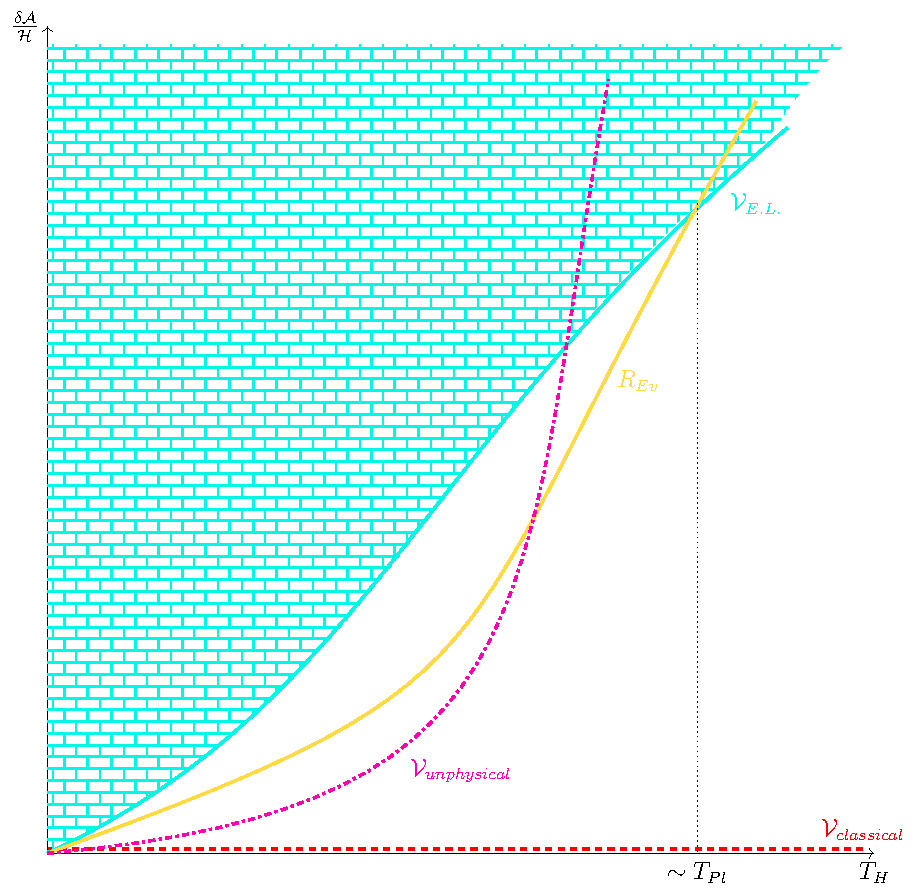
\includegraphics[scale=0.77]{Immagini/state-independent-bounds/state-independent-bounds.pdf}
	\caption[]{representation of the idea at the base of section \ref{subsec:state-independent-bounds}. We expect any physical bound to grow faster than the expected black hole evaporation rate, at least in the region \(T \lesssim T_{Pl}\). Energy conditions leading to bounds that do not share this feature would lead to similar problems as the classical area theorem; we therefore would try to rule out those energy conditions, believed unphysical.}
	\label{fig:state-independent-bounds}
\end{figure}

\subsection{Singularity theorems}

Let us finally present a small result, interesting for the application of singularity theorems. In order to explain it, it is necessary for us to venture on a quick journey to how a singularity theorem can be proved by means of index form methods. This is the central topic of the article we have mainly been referring to, namely \cite[]{fewster2020new}, so we will proceed to take a quick review of it.

According to Senovilla \cite[]{senovilla1998singularity}, a singularity theorem needs three main ingredients:
\begin{itemize}
	\item[\ding{99}] A causality condition, typically global hyperbolicity, or, following Minguzzi, past reflectivity and openess.
	\item[\ding{99}] An energy condition, of the like we have already been discussing enough about in chapter \ref{ch:energy-conditions}.
	\item[\ding{99}] A boundary or initial condition.
\end{itemize}
It is precisely of this last ingredient that we are going to discuss in this section.
The classical Penrose singularity theorem relies on global hyperbolicity, the null energy condition and the presence of a future trapped surface, as the ones defined in \ref{def:trapped-surface}. Precisely, it states
\begin{theorem}
	Any globally hyperbolic spacetime \((M,g)\), where the null energy condition holds everywhere and it contains a trapped surface cannot be future null geodesically complete, or, in other words, it contains at least one incomplete causal geodesic.
\end{theorem}

\begin{proof}
	A sketch of the proof proceeds as follows: suppose that \(M\) is geodesically complete and consider its trapped surface \(P\). Take any congruence of null geodesics leaving normally from \(P\); by means of criteria \ref{prop:fp-criteria} (it is enought to choose the same set of functions \(\mathcal{A}_{NEC}\) used in \ref{th:classical-bh-area}) it is possible to show that any congruence must develop a focal point within distance \(L_{\hat{\mathrm{H}}} = \frac{1}{\vert \mathrm{H} \vert}\) from the manifold \(P\), which is in contradiction with the supposed geodesic completeness.
\end{proof}
 
It is immediate to spot out that here the \emph{initial condition} mentioned in Senovilla's structure is nothing but the presence of a trapped surface, or better, of a surface whose mean normal curvature is such that:
\[
\mathrm{H}^{\mu}U_{\mu} < 0,
\]
for all \(U^{\mu}\) future pointing null vectors.
In Wald \cite[]{wald2010general} and Hawking and Ellis \cite[]{hawking1973large} it was already present a theorem stating that trapped surfaces, under the validity of the null energy condition, had to be hidden beyond the horizion, an observation which is clear here given that for theorem \ref{th:classical-bh-area} any surface outside the horizon must fulfill \(\mathrm{H}^{\mu}U_{\mu} \ge 0\).

With the possibility of an evaporating horizion this is not true anymore, as surfaces outside the horizion are allowed to shrink too. However, under the weaker energy conditions that allow an horizion to evaporate, the intial condition to prove a singularity theorem must be strengthened, namely it is not enough anymore to start from a trapped surfaced, but a ``sufficiently trapped'' surface is needed (see \cite[]{fewster2020new}). Is it possible then to find such surfaces outside the horizion? Well, naturally the answer is no.
\begin{prop}
	Any surface giving the sufficient initial condition to prove the formation of a singularity must lay in the black hole region.
\end{prop}

\begin{proof}
	Focal points form along every othogonal null geodesic leaving from a codimension \(2\) surface \(P\) if and only if equation \eqref{eq:fp-criteria} holds for any \(U^{\mu}\). However, outside the horizion the null generators of the boundary of the future of \(P\) must satisfy the opposite inequality because of the definition of horizion itself. Hence, any surface \(P\) satsifying such criteria must lay in the black hole region.
\end{proof}

This is a generalization of proposition \(12.2.3\) of \cite{wald2010general}, but notice that, where Wald needs to ask for the null energy condition to hold, here no enwegy condition is required: this is indeed only a statement of geometric properties of the spacetime, the energy condition is only needed to estimate ``how far'' the black hole region extends.

Such a result is in accordance with the already mentioned proof of singularity theorems for evaporating black holes given in \cite[]{freivogel2020return}. In that article the authors also proceed to estimate how fare into the black hole they might need to go in order to find the required trapped surface. In some sense, that distance can be turned into a measure of ``how accurate'' is the energy condition that has been applied: the smaller the distance, the less information has been wahsed out and hence the strongest is the theorem.

\clearpage

\chapter{Singularity Theorems}
\label{ch:singularity-theorems} 

Penrose Singularity Theorem....

\begin{remark}
    Notice that the bound on the initial condition required for any singularity theorem is exactly complementary to the one set by the area theorem, as they are based on the same property of the functional \(J[f]\).

    In particular then, whatever surface used as initial condition for a singularity theorem will have to be entirely contained within the black hole horizion.
    This is actually a generalization of proposition \(12.2.3\) of \cite{wald2010general} to weaker energy conditions.
\end{remark}

	
	
	
	
	
	

	
	
	
	
	






\printbibliography


\end{document}          
